% Options for packages loaded elsewhere
\PassOptionsToPackage{unicode}{hyperref}
\PassOptionsToPackage{hyphens}{url}
  %
\documentclass[
   11pt,
       ]{book}
  \usepackage{amsmath,amssymb}
  \usepackage{lmodern}
  \usepackage{setspace}
 \usepackage{iftex}
\ifPDFTeX
\usepackage[T1]{fontenc}
\usepackage[utf8]{inputenc}
\usepackage{textcomp} % provide euro and other symbols
\else % if luatex or xetex
  \usepackage{unicode-math}
 \defaultfontfeatures{Scale=MatchLowercase}
\defaultfontfeatures[\rmfamily]{Ligatures=TeX,Scale=1}
 \setmainfont[]{SourceSerifPro-Regular}
  \setsansfont[]{SourceSansPro-Regular}
  \setmonofont[]{SourceCodePro-Regular}
      \fi
  % Use upquote if available, for straight quotes in verbatim environments
\IfFileExists{upquote.sty}{\usepackage{upquote}}{}
\IfFileExists{microtype.sty}{% use microtype if available
 \usepackage[]{microtype}
 \UseMicrotypeSet[protrusion]{basicmath} % disable protrusion for tt fonts
}{}
 \makeatletter
\@ifundefined{KOMAClassName}{% if non-KOMA class
 \IfFileExists{parskip.sty}{%
  \usepackage{parskip}
 }{% else
  \setlength{\parindent}{0pt}
  \setlength{\parskip}{6pt plus 2pt minus 1pt}}
}{% if KOMA class
 \KOMAoptions{parskip=half}}
\makeatother
  \usepackage{xcolor}
\IfFileExists{xurl.sty}{\usepackage{xurl}}{} % add URL line breaks if available
\IfFileExists{bookmark.sty}{\usepackage{bookmark}}{\usepackage{hyperref}}
\hypersetup{
                                  hidelinks,
               pdfcreator={LaTeX via pandoc}}
\urlstyle{same} % disable monospaced font for URLs
   \usepackage[margin=2.5cm]{geometry}
           \usepackage{longtable,booktabs,array}
   \usepackage{calc} % for calculating minipage widths
   % Correct order of tables after \paragraph or \subparagraph
 \usepackage{etoolbox}
 \makeatletter
 \patchcmd\longtable{\par}{\if@noskipsec\mbox{}\fi\par}{}{}
 \makeatother
 % Allow footnotes in longtable head/foot
 \IfFileExists{footnotehyper.sty}{\usepackage{footnotehyper}}{\usepackage{footnote}}
 \makesavenoteenv{longtable}
               \setlength{\emergencystretch}{3em} % prevent overfull lines
   \providecommand{\tightlist}{%
    \setlength{\itemsep}{0pt}\setlength{\parskip}{0pt}}
       \setcounter{secnumdepth}{5}
                             \usepackage{booktabs}
\usepackage{graphicx}
\usepackage[font=small,labelfont=bf]{caption}

\usepackage{enumitem}
\setlist[itemize,1]{label={---}}
\usepackage{subcaption}
\usepackage{tipa}
\usepackage{empheq}

\definecolor{ptol1}{HTML}{4477AA}
\definecolor{ptol2}{HTML}{CC6677}
\newcommand{\reg}{\color{ptol1}}
\newcommand{\irr}{\color{ptol2}}
\usepackage{booktabs}
\usepackage{longtable}
\usepackage{array}
\usepackage{multirow}
\usepackage{wrapfig}
\usepackage{float}
\usepackage{colortbl}
\usepackage{pdflscape}
\usepackage{tabu}
\usepackage{threeparttable}
\usepackage{threeparttablex}
\usepackage[normalem]{ulem}
\usepackage{makecell}
\usepackage{xcolor}
\ifLuaTeX
  \usepackage{selnolig}  % disable illegal ligatures
\fi
\usepackage[]{natbib}
\bibliographystyle{apalike}

\author{}
\date{}


% Begin stuff for thesis format, partially adapted from:
% https://www.overleaf.com/latex/templates/mit-thesis-template/ytphktgwpktc
\pagestyle{plain}

\def\titlepage{\cleardoublepage\centering
  \thispagestyle{empty}
  \parindent 0pt \parskip 10pt plus 1fil minus 1fil
  \def\baselinestretch{1}\normalsize\vbox to \vsize\bgroup\vbox to 9in\bgroup}
\def\endtitlepage{\par\kern 0pt\egroup\vss\egroup\newpage}

\def\permission{\par\noindent{\centering
   The author hereby grants to MIT permission to reproduce and to
   distribute publicly paper and electronic copies of this thesis
   document in whole or in part in any medium now known or hereafter
   created.}\par}

\def\signature#1#2{\par\noindent#1\dotfill\null\\*
  {\raggedleft #2\par}}
  
\def\abstract{\subsection*{Abstract}\small\def\baselinestretch{1}\normalsize}

% heading font
\usepackage{sectsty}
\allsectionsfont{\sffamily}

% TOC
\usepackage[nottoc]{tocbibind}
\usepackage{tocloft}
% \renewcommand{\cftpartfont}{\normalfont\sffamily\bfseries}% \part font in ToC
\renewcommand{\cfttoctitlefont}{\sffamily\huge}
% \renewcommand{\cftdot}{\ensuremath{\cdot}}
% \cftsetpnumwidth{1em}

% \renewcommand{\cftchappresnum}{Chapter }
% \renewcommand{\cftchapaftersnumb}{\\}
% \setlength{\cftchapnumwidth}{5.5em}
\renewcommand{\cftchapfont}{\sffamily\large}
\renewcommand{\cftchappagefont}{\sffamily\large}
\renewcommand{\cftchapdotsep}{\cftnodots}
% \renewcommand{\cftchapdotsep}{2}

\renewcommand{\cftsecfont}{\sffamily\slshape}
\cftpagenumbersoff{section}
% \renewcommand{\cftsecpagefont}{\sffamily}
% \renewcommand{\cftsecdotsep}{\cftnodots}

% \renewcommand{\cftsubsecfont}{\normalfont\itshape}
% \renewcommand{\cftsubsubsecfont}{\normalfont\small}

\begin{document}

% removed default pandoc stuff:
% % 
% Thesis format -- title page
\begin{titlepage}
\large
{\def\baselinestretch{1.2}\Large\bf Language learning at scale: Data-driven and model-motivated analyses of lexical and morphological development \par}
by\par
{\Large Mika Braginsky}\par
B.S., Massachusetts Institute of Technology (2014)\par\vspace{1em}
Submitted to the Department of Brain and Cognitive Sciences \\
in partial fulfillment of the requirements for the degree of\par
Doctor of Philosophy in Brain and Cognitive Sciences\par
at the\par
Massachusetts Institute of Technology \par
February 2022\par
% copyright: \copyright 2022 Mika Braginsky. All rights reserved. \permission
\copyright\ Mika Braginsky 2022. All rights reserved. \permission \par
\vskip 3\baselineskip
\signature{Author}{Department of Brain and Cognitive Sciences \\ January 31st, 2022}\par\vfill
\signature{Certified by}{Edward Gibson \\ Professor, Brain and Cognitive Sciences \\ Thesis Supervisor}\par\vfill
\signature{Accepted by}{Mark Harnett \\ Graduate Officer, Department of Brain and Cognitive Sciences}\vfill
\end{titlepage}
%

% Thesis format -- abstract page
\cleardoublepage
\begin{center}{\large{\bf Language learning at scale: Data-driven and model-motivated analyses of lexical and morphological development} \\[\baselineskip]
by \\[\baselineskip]
Mika Braginsky \\[2\baselineskip]}
\par
% \def\baselinestretch{1}\normalsize
Submitted to the Department of Brain and Cognitive Sciences \\
on January 31st, 2022, in partial fulfillment of the requirements \\
for the degree of Doctor of Philosophy in Brain and Cognitive Sciences \\[3\baselineskip]
\end{center}
\par
\begin{abstract}
\input{abstract.txt}
\end{abstract}
\par
\noindent
\vskip\baselineskip
Thesis Supervisor: Edward Gibson \\ Title: Professor, Brain and Cognitive Sciences
% \newpage
%

% Thesis format -- acknowledgements
% \cleardoublepage
% \section*{Acknowledgements}
% \def\baselinestretch{1}\normalsize
% \input{acknowledgements.txt}

{
\setcounter{tocdepth}{1}
\tableofcontents
}
\setstretch{1.5}
\hypertarget{intro}{%
\chapter{Introduction}\label{intro}}

Imagine you're a baby, eager to make sense of the bewildering world around you. From the sea of sounds surrounding you, you start picking out repeated pieces. Aha! your long-haired companion can be called a \emph{doggie}. You rapidly add to your collection --- that thing is a \emph{banana}, someone can \emph{eat} it, people say \emph{hi} to one another. Before too long you've started putting these bits together --- \emph{hi doggie!} --- and changing them to suit your needs --- \emph{doggie eating bananas}. By the time you're out of diapers, you've learned hundreds of words and can combine them in ever more complex ways.

Now imagine that you're a scientist, eager to understand how this remarkable learning process unfolded. You might wonder, why was \emph{doggie} learned before \emph{banana} and before \emph{eat}? How did these distinct words come to be joined by combinations and modifications such as \emph{doggies} and \emph{bananas} and \emph{doggies ate bananas}? What happened when \emph{doggie} was overzealously said to have \emph{eated}?

To get any traction on these questions, you'll need to take into account that the child's abilities and knowledge were ever-changing throughout this process. And while this particular sequence occurred for this one child, there is tremendous variation in individual children's linguistic journeys. Moreover, these words and structures are in a specific language, and we need to understand how any of the many and varied languages of the world can be learned using the same underlying machinery.

In this thesis, I investigate lexical and morphological development, i.e.~how young children learn words and word structures. I use dense datasets and computational models to find generalizations (1) across children, (2) over the course of development, and (3) among various languages. In the rest of this introductory chapter, I first briefly introduce the main data source used in my studies --- the MacArthur-Bates Communicative Development Inventory \citep{fenson2007} as aggregated in Wordbank \citep{frank2017}. I then outline why these three dimensions of scale matter and what strengths and weaknesses various data sources have with respect to them. Finally, I give an overview of three completed studies, and a series of proposed future studies, of language learning at scale.

The MacArthur-Bates Communicative Development Inventory (CDI) is a checklist for parents to fill out to report on their child's progress in learning language through the first three years of their life. In different versions of the form, parents mark whether their child ``says'' or ``understands and says'' particular words and word forms out of a list of several hundred. CDI forms have been adapted to dozens of languages. Because the CDI is standardized and inexpensive to administer, data from thousands of children has been collected by various research labs around the world.

To take advantage of the opportunity presented by the wide adoption of the CDI, my collaborators and I created Wordbank, an open repository that aggregates administrations of the CDI across languages. Wordbank contains around 83,000 administrations of CDIs in 30 languages, enabling a variety of novel analyses of language learning at scale. We believe this database is the largest and most diverse set of data on early language acquisition currently in existence.

For each of the three dimensions of scale listed above --- across children, over development, and among languages --- I describe below how the data from various sources can and can't contribute to these directions of generalization. Historically, the main empirical methods in the study of language learning have been diary studies, in-lab experiments, naturalistic observation (audio recordings in the lab or home), and parent report surveys such as the CDI. Each method has been fruitful in building knowledge about children's language learning, though each has its strengths and weaknesses in terms of the richness of their data.

\textbf{Generalizing across children}. Children vary enormously in rates of vocabulary development \citep{fenson1994, frank2021} and in the routes they take during language learning \citep{nelson1973, bates1991, bates1994, frank2021}. Given this large amount of individual variation, we need large sample sizes both to generalize across children and to study the degree to which learning processes are idiosyncratic vs.~standardized. Diary studies are generally focused on just one child. In-lab studies study groups of children, but sample sizes are for the most part small, given the cost and time needed to conduct experiments. Small sample sizes result in many studies being under-powered, contributing to over-inflated, non-reproducible effects \citep{button2013, osc2012}. Naturalistic recording datasets can have many subjects, but of course cost increases with sample size, especially because of the enormous labor intensiveness of transcription. Studies tend to lie on a trade-off between having a smaller number of subjects and a lot of data per subject -- at the extreme, the Speechome project with one subject and nearly constant audio recording \citep{roy2015} -- or a larger number of subjects with less data per subject (as is the case for most corpora in the CHILDES repository, which have between 1 and 42 subjects \citep{macwhinney2000}). Conversely, the CDI is relatively much cheaper to administer, so CDI datasets tend to have hundreds or thousands of subjects.

\textbf{Characterizing development}. In-lab studies typically test either one group of children of a roughly similar age, or two or three groups of children, each of roughly similar age. The resulting claim is thus about children's abilities at a broad age bin, e.g.~``3 year olds can do X'', or a comparison of the abilities of children from several age bins, e.g.~``3 year olds can't do X but 4 year olds can, so X emerges between 3 and 4 years''. This is at best a very rough estimate of the age at which an ability may have developed in the average child, and not fine-grained enough to provide a detailed developmental trajectory, for individuals or in the aggregate. Diary studies and naturalistic recordings often measure children at much finer time points, collecting data anywhere from daily to every few weeks to every six months. However, typical sampling rates result in capturing only a tiny fraction of a child's total language output, making inferences about the onset or development of particular language phenomena very hard \citep{tomasello2004}. In the CDI, children are generally binned by month, so cross-sectional data gives information at one-month granularity, and longitudinal data gives information at a few-month granularity -- the length of the form means that it's not administered more often. In combination with large sample sizes, this allows for detailed developmental trajectories.

\textbf{Comparing and contrasting languages}. Given the enormous diversity of the world's languages, for theories to generalize across languages, they need to be informed by data from many languages. Otherwise, we risk generating theories of language learning that only apply to a subset of languages and don't enable us to understand language learning as a universal process. Since diary studies and naturalistic recordings are conducted on a per-child basis, the resulting data are in a single language (except in cases where the child is multilingual). In-lab studies also tend to be in a single language, although experiments using novel words or artificial grammars can in some ways sidestep the single-language specificity. For both kinds of data, comparing across studies in different languages, even if the phenomena under investigation are similar, is very challenging. Additionally, since studies tend to build on one another, subfields can become overly focused on specific phenomena. For example, much of the study of morphology learning focuses on how children learn the English past tense, which is a useful case study but is hardly prototypical across languages. However, the CDI has been adapted to many languages, and disparate datasets from around the world are now aggregated in the Wordbank repository \citep{frank2017}. Although there are challenges with the idiosyncrasies of different CDI forms and samples, this now allows for a wide range of fruitful cross-linguistic comparison \citep{braginsky2019, frank2021}.

In addition to the three data-related desiderata described above, it's vital to consider how different data sources do and don't allow us to distinguish among theories. The connection between empirical data and theoretical predictions is key to adjudicating between competing accounts of language learning. With CDI data, it can be challenging to form clear links to theory, since measurement is limited to the set of items on a standardized checklist. In-lab experiments, on the other hand, allow for carefully designed stimuli and measures that allow researchers to compare different hypotheses. In both cases, however, theories must be properly fleshed out to provide clear, testable predictions. For example, a long-time theoretical controversy has centered on the learning of the English past tense, with a dichotomy between ``dual-route'' (having separate representations for regular and irregular verbs) and ``single-route'' (having a unified representation for both) accounts. Throughout, researchers on both sides of the debate have made strong claims about the nature of mental representations, often without determining directly comparable, quantitative predictions of the various accounts. For example, evidence for commonality in how regular and irregular verbs are processed was taken as evidence against a dual-route system (and by extension against symbolic rules), but a system with graded, probabilistic application of rules could potentially be consistent with this data. Conversely, many claims about what single-route, neural network models could or could not in principle learn were subsequently disproven by a new model's success \citep{macwhinney1991, plunkett1991, plunkett1993, westermann1995, hoeffner1996, nakisa1996, plunkett1997, plunkett1999, hahn2000}. Such accounts need to be cached out into computational models to be fully specified enough for their assumptions and predictions to be compared on equal footing.

To summarize the discussion above, CDI datasets support cross-linguistic analyses with large samples and detailed developmental trajectories. However, their connection to theory is somewhat indirect and their temporal density can be limited. As such, the studies in this thesis first draw on the strengths of CDI data to investigate lexical development (Chapter \ref{aoa-pred}), morphological development (Chapter \ref{cdi-overreg}), and the relationship between them (Chapter \ref{cdi-overreg}). I next turn to a computational modeling simulation paradigm to make detailed comparisons between models of morphological productivity (Chapter \ref{prod-comp}). In the conclusion, I propose using a novel method of data collection to create a rich dataset on morphological development that can be used to quantitatively evaluate theories of morphology learning (Chapter \ref{conclusion}).

First, in Chapter \ref{aoa-pred} (published as \citet{braginsky2019}), we investigate lexical development by asking which properties of words make them easier or harder to learn. We use CDI data from thousands of children to estimate the learning trajectories of hundreds of words in ten languages, and predict these trajectories based on word-level properties of their meaning and linguistic environment. We examine the effects of these properties and the extent to which they are consistent or variable for several languages and lexical categories.

For the rest of the studies in this thesis, I focus on morphology learning. In Chapter \ref{cdi-overreg} we ask how lexical development relates to morphological development. We use large CDI datasets in three languages to evaluate how children's production of correct past tense forms of irregular verbs (ate) and overregularizations (eated) is driven by their vocabulary size, age, and combination of the two. We also use longitudinal data to examine individual children's developmental trajectories of overregularization.

Chapter \ref{prod-comp} also centers on morphology learning, but through a different lens. We use a computational simulation paradigm to investigate the similarities and differences among several leading models of morphological generalization. We perform this comparison using a space of language-agnostic, parametrically-varying corpora. Through a series of analyses, we show that these models make systematically differing predictions about morphological generalization, and we ascertain which assumptions of the models are critical to these differences.

Lastly, in Chapter \ref{conclusion} I lay out a proposal for creating a rich dataset on the morphological development of a large sample of children and using these data to quantitatively evaluate theories of morphology learning. First, the planned cross-sectional study will assess which properties of words influence their propensity to be overregularized and irregularized. Next, a larger, longitudinal study will allow us to characterize the developmental trajectories of (over)generalization for individual children and words. Finally, instantiating theories of morphology into comparable computational models will allow us to test each theory quantitatively on equal footing, and meaningfully compare between proposals using the data from the two studies.

Taken together, these studies synthesize empirical and computational methods to investigate multiple domains of language development at scale. Focusing on lexical and morphological development, they clarify and enhance the empirical and theoretical landscape of language learning.

\hypertarget{aoa-pred}{%
\chapter{Consistency and variability in word learning across languages}\label{aoa-pred}}

\hypertarget{introduction}{%
\section{Introduction}\label{introduction}}

Despite tremendous individual variation in children's rate of development \citep{fenson2007}, the first words that they utter are strikingly consistent \citep{tardif2008,schneider2015}: they tend to talk about important people in their life (``mom'', ``dad''), social routines (``hi'', ``uh-oh''), animals (``dog'', ``duck''), and foods (``milk'', ``banana''). Even as children learn from their own experiences and according to their own interests \citep{mayor2014,nelson1973}, their vocabulary grows rapidly, typically adding more nouns, but also verbs (``go'') and other predicates (``hot'') to their repertoires. Over just their first three years, children learn hundreds, even thousands of words \citep{fenson1994,mayor2011}.

One classic approach to word learning focuses on the specific mechanisms that children bring to bear on the learning problem. For example, across many laboratory experiments, a variety of mechanisms have been identified as plausible drivers of early word learning, including co-occurrence based and cross-situational word learning \citep{schwartz1983,yu2007}; social cue use \citep{baldwin1993}; and syntactic bootstrapping \citep{gleitman1990,mintz2003}. The ability to identify which of these mechanisms is most explanatory has been challenging. Indeed, many theories of early word learning take multiplicity of cue types and mechanisms as a central feature (e.g., \citealp{hollich2000,bloom2000}). As important as this work is, though, these studies are typically aimed at understanding how one or a small handful of words are learned in the laboratory under precisely-defined learning conditions. They do not directly address questions regarding the developmental composition and ordering of growth in the lexicon across many different children in their natural environments, nor whether these patterns are consistent across different languages.

An alternate approach to word learning asks why some words are learned so early and some much later. This question about the order of the acquisition of first words can provide a different window into the nature of children's language learning. Posed as a statistical problem, the challenge is to find what set of variables best predicts the age at which different words are acquired. Previous work using this approach has revealed that, in English, within a lexical category (e.g., nouns, verbs), words that are more frequent in speech to children are likely to be learned earlier \citep{goodman2008}. Further studies have found evidence that a variety of other semantic and linguistic factors are related to word acquisition, such as salience and iconicity \citep{hills2009,stokes2010,perry2015,roy2015,swingley2017}.

But these exciting findings are limited in their generality because each study used a different dataset and focused on different predictors. In addition, nearly all studies to date have exclusively analyzed data from English-learning children, providing no opportunity for cross-linguistic comparison of the relative importance of the many relevant factors under consideration. Cross-linguistic comparisons are critical to identifying the universal mechanisms that are in play for all children and differentiating them from patterns of acquisition that emerge due to the particulars of a given language or culture \citep{slobin1985,bates1987}. Our goal here is to extend these classic approaches by assessing the degree to which the predictors of word learning are consistent across different languages, as well as whether there are similar patterns across different lexical categories.

The primary tool for characterizing the breadth of children's early vocabularies in these previous studies has been structured parent report. Naturalistic language samples and experimental methods are both valuable methods for assessing aspects of child language \citep{bornstein1998,fernald2006}. But outside of a few ultra-dense transcripts (e.g., \citealp{roy2015}), neither method typically provides the kind of holistic and comprehensive view that comes from parent report. We focus in particular on the MacArthur-Bates Communicative Development Inventory (CDI; \citealp{fenson2007}), a family of parent-report vocabulary checklists in which parents are asked whether their child ``understands'' or ``understands and says'' a large set of individual words.

The CDIs are an inexpensive and widely-used method for gathering reliable and valid data about the nature and extent of young children's productive and receptive vocabularies (see \citealp{fenson1994} for review; cf.~\citealp{feldman2000, fenson2000}). Although CDIs cannot exhaustively capture all words in a child's vocabulary \citep{mayor2011}, they do give an estimate of a child's knowledge about several hundred words, far more than the handful that are typically tested in a lab experiment. CDI estimates of vocabulary size are highly correlated with children's vocabulary knowledge as assessed with naturalistic observation or using standardized tests \citep{fenson2007}. Of course, any parent report measure is subject to reporting biases. The CDIs were designed to minimize these by asking parents to report only on observable behaviors that are currently (rather than retrospectively) demonstrated and to identify words from a pre-selected list (rather than having them recall them on their own).

Because of the low cost of administering CDI instruments, it is relatively easy to gather samples containing data about hundreds or thousands of children. Such large samples in turn make it possible to recover stable estimates of the average difficulty of individual words, even if individual children's data may be noisy. Thus, CDI data are typically the dataset of choice for the studies of vocabulary composition described above.

Finally, CDI instruments have been adapted in dozens of different languages, providing an opportunity for cross-linguistic comparison. The American English CDI is not simply translated to other languages verbatim; instead, expert groups of researchers adapt the form for their particular linguistic and cultural situation. This process leads to a wide range of forms that share a common structure, but contain sets of words that are customized to a particular language and culture. Thus, cross-linguistic comparisons do not reflect children's acquisition of a single set of words, but instead capture relevant information regarding patterns of children's vocabulary development using instruments designed specifically for each language.\footnote{Of course, observational data of this type are still open to other sources of bias, a point we return to in the Discussion.}

In our study, we conduct cross-linguistic comparisons of the acquisition trajectories of children's early-learned words using Wordbank (\href{http://wordbank.stanford.edu}{wordbank.stanford.edu}; \citealp{frank2017}), an open repository that aggregates administrations of the CDI across languages. We integrate these acquisition trajectory data with independently-derived characterizations of the word learning environment from other datasets. The use of secondary datasets is warranted because no currently available resource provides data on both children's language environments and their learning outcomes for more than a small handful of children. In particular, we derive our estimates of the language environment from transcripts of speech to children in the CHILDES database \citep{macwhinney2000} and measures of meaning-related word properties from available psycholinguistic databases. This data-integration methodology was originated by \citet{goodman2008}; it relies on large samples to average out the (substantial) differences among children and care environments. While introducing additional sources of variability, this approach allows for analyses that cannot be performed on smaller datasets that measure only children or environments but not both.

To measure environmental input, we used existing adult speech data from the CHILDES database to estimate each word's frequency (a) in speech to children, (b) as a sole utterance constituent, (c) in utterance-final position, and the (d) mean length in words of utterances (MLU-w) containing that word. While crude, these measures are both easy to compute and relatively comparable across languages. To derive proxies for the meaning-based properties of each word, we accessed available psycholinguistic norms using adult ratings of each word's (a) concreteness, (b) valence, (c) arousal, and (d) association with babies. Integrating these estimates, we predict each word's acquisition trajectory, assessing the relative contributions of each predictor, how predictors change over development, and how predictors differ by lexical category. Since vocabulary composition differs in comprehension and production (e.g., \citealp{benedict1979}), we conduct our analyses independently on each.

These analyses address two questions. First, we ask about the degree of consistency across languages in the relative importance of each predictor. To do so, we compare the estimates for the effect of each predictor for each language and conduct analyses that determine the likelihood that the consistency of the estimates did not occur by chance. Consistency in the patterning of predictors would suggest that similar information sources are important for learners, regardless of language, and that linguistic dissimilarities (e.g., greater morphological complexity in Russian, greater phonological complexity in Danish) do not dramatically alter the course of acquisition. Conversely, evidence for variability across languages would show the degree to which learners face different challenges in learning different languages, posing a challenge for more universalist accounts. Further, systematicity in the variability between languages would reveal which languages are more similar than others in the structure of these different challenges.

Second, we ask which lexical categories are most influenced by linguistic environment factors, like frequency and utterance length, compared with meaning-based factors like concreteness and valence. Division of dominance theory suggests that nouns might be more sensitive to meaning factors, while predicates and closed-class words might be more sensitive to linguistic environment factors \citep{gentner2001}. And on syntactic bootstrapping theories \citep{gleitman1990}, nouns are argued to be learned via frequent co-occurrence (operationalized by frequency) while verbs might be more sensitive to syntactic factors (operationalized here by utterance length; \citealt{snedeker2007}). Thus, examining the relative contribution of different predictors across lexical categories can help test the predictions of influential theories of acquisition.

\hypertarget{methods}{%
\section{Methods}\label{methods}}

\hypertarget{acquisition-trajectories}{%
\subsection{Acquisition trajectories}\label{acquisition-trajectories}}

To estimate the trajectory of words' acquisition, we used vocabulary data collected using CDI instruments adapted in many different languages, including both Words \& Gestures (WG) and Words \& Sentences (WS) forms. When filling out a CDI form, parents are either asked to indicate whether their child ``understands'' (comprehension) or ``understands and says'' (production) each of around 400-700 words. Both comprehension and production are queried for younger children and only production is queried for older children. We included data from the items on the WG form for comprehension, and data from the items in common between the WG and WS forms for production. Placeholder items, such as ``child's own name,'' were excluded. Table~\ref{tab:langstats} gives an overview of our acquisition data (\citealp{kovacevic1996,bleses2008,boudreault2007,trudeau2011,caselli2012,caselli1995,simonsen2014,vershinina2011,eliseeva2009,fenson2003,eriksson2002,acarlar2008}.
Each of the datasets was collected in the language of the community, e.g., the Mexican Spanish CDI data were collected in several areas of Mexico; longitudinal administrations were excluded.

\begin{table}

\caption{\label{tab:langstats}Statistics for data from Wordbank and CHILDES. N indicates number of children.}
\centering
\begin{tabular}[t]{>{}lrrlrlrr}
\toprule
\multicolumn{1}{c}{} & \multicolumn{1}{c}{} & \multicolumn{2}{c}{Production} & \multicolumn{2}{c}{Comprehension} & \multicolumn{2}{c}{CHILDES} \\
\cmidrule(l{3pt}r{3pt}){3-4} \cmidrule(l{3pt}r{3pt}){5-6} \cmidrule(l{3pt}r{3pt}){7-8}
Language & CDI items & N & Ages & N & Ages & Types & Tokens\\
\midrule
\textbf{Croatian} & 388 & 627 & 8-30 & 250 & 8-16 & 12,064 & 218,775\\
\textbf{Danish} & 381 & 6,112 & 8-36 & 2,398 & 8-20 & 4,956 & 195,658\\
\textbf{English (American)} & 393 & 7,312 & 8-30 & 1,792 & 8-18 & 45,597 & 7,679,042\\
\textbf{French (Quebec)} & 396 & 1,364 & 8-30 & 537 & 8-16 & 28,819 & 2,551,113\\
\textbf{Italian} & 392 & 1,400 & 7-36 & 648 & 7-24 & 7,544 & 188,879\\
\textbf{Norwegian} & 380 & 7,466 & 8-36 & 2,374 & 8-20 & 10,670 & 231,763\\
\textbf{Russian} & 410 & 1,805 & 8-36 & 768 & 8-18 & 5,191 & 32,398\\
\textbf{Spanish (Mexican)} & 399 & 1,891 & 8-30 & 788 & 8-18 & 33,529 & 1,609,614\\
\textbf{Swedish} & 371 & 1,367 & 8-28 & 467 & 8-16 & 8,815 & 359,155\\
\textbf{Turkish} & 395 & 3,537 & 8-36 & 1,115 & 8-16 & 6,503 & 44,347\\
\bottomrule
\end{tabular}
\end{table}

For each word, the CDI data yield a trajectory reflecting the number of children that are reported to understand or produce the word at each age covered by the instrument (see Figure~\ref{fig:aoapred-demotraj} for some examples).



\begin{figure}

{\centering \includegraphics[width=\textwidth]{thesis-mikabr_files/figure-latex/aoapred-demotraj-1} 

}

\caption{Example production trajectories for the words ``dog'' and ``jump'' across languages. Points show the proportion of children producing each word for each one-month age group. Lines show the best-fitting logistic curve. Labels show the forms of the words in each language.}\label{fig:aoapred-demotraj}
\end{figure}

\hypertarget{word-properties}{%
\subsection{Word properties}\label{word-properties}}

For each word in each of our 10 languages, we used corpora of child-directed speech in that language from CHILDES to obtain an estimate of its frequency, the mean length of utterances in which it appears, its frequency as the sole constituent of utterance, and its frequency in utterance final position. We also computed each word's length in phonemes.

In addition, each word's concreteness, valence, arousal, and relatedness to babies\footnote{Previous studies have shown robust consistency in the types of words that children learn very early \citep{tardif2008}. These words seem to describe concepts that are important or exciting in the lives of infants in a way that standard psycholinguistic features like concreteness do not. Capturing this intuition quantitatively is difficult, but \citet{perry2015} provide a proxy measure as a first step. This measure is simply the degree to which a particular word was ``associated with babies''. Intuitively, we expect this measure to capture the degree to which words like ``ball'' or ``bottle'' feature heavily in the environment (and presumably, mental life) of many babies.} were compiled from ratings based on previous studies using adult raters. Since existing ratings are primarily available for English, we mapped all words onto translation equivalents across CDI forms, verified by native speaker judgement, allowing us to use the English ratings across languages. Of the resulting translation equivalent meanings, 35\% occur only in one language, 51\% occur in more than one but not all languages, and 14\% occur in all languages. While necessarily imperfect, this method allows us to examine languages for which limited resources exist. Example words for these predictors in English are shown in Table~\ref{tab:extremes}.

\begin{table}

\caption{\label{tab:extremes}Items with the highest and lowest values for each predictor in English.}
\centering
\resizebox{\linewidth}{!}{
\begin{tabular}[t]{lll}
\toprule
Predictor & Highest & Lowest\\
\midrule
Arousal & naughty, money, scared & today, asleep, shh\\
Babiness & baby, bib, bottle & jeans, penny, donkey\\
Concreteness & apple, baby, ball & that, now, how\\
Final frequency & book, it, there & put, when, give\\
Frequency & you, it, that & babysitter, rocking chair, grrr\\
MLU-w & daddy, when, day & ouch, thank you, peekaboo\\
Number phonemes & refrigerator, cockadoodledoo, babysitter & i, eye, ear\\
Solo frequency & no, yes, thank you & feed, bathroom, tooth\\
Valence & happy, hug, love & ouch, hurt, sick\\
\bottomrule
\end{tabular}}
\end{table}

Each numeric predictor was centered and scaled (within language) so that all predictors would have comparable units.

\textbf{Frequency}. For each language, we derived unigram counts based on adult speech in all corpora in CHILDES for that language. Frequencies varied widely both within and across lexical categories.
Each word's count was summed across inflected forms (e.g., ``dogs'' counts as ``dog'') and synonyms (e.g., ``father'' counts as ``daddy''). For polysemous words (e.g., ``orange'' as in color or fruit), occurrences were split uniformly between the senses on the CDI (there were only between 1 and 10 such word pairs in the various languages; in the absence of cross-linguistic corpus resources for sense disambiguation, this is a necessary simplification). Counts were normalized to the length of each corpus, Laplace smoothed (i.e., counts of 0 were replaced with counts of 1), and log transformed.

\textbf{Solo and Final Frequencies}. Using the same dataset as for frequency, we estimated the frequency with which each word occurred as the sole word in an utterance, and the final word of an utterance (not counting single-word utterances). Solo and final counts were normalized to the length of each corpus, Laplace smoothed, and log transformed. Since both of these estimates are by necessity highly correlated with frequency, we then residualized unigram frequency out of both, so that values reflect an estimate of the effects of solo frequency and final frequency over and above frequency.

\textbf{MLU-w}. MLU-w is only a rough proxy for syntactic complexity, but is relatively straightforward to compute across languages (in contrast to other metrics). For each language, we estimated each word's MLU-w by calculating the mean length in words of the utterances in which that word appeared, for all corpora for that language. For words that occurred fewer than 10 times, MLU-w estimates were treated as missing.

\textbf{Number of phonemes}. In the absence of consistent resources for cross-linguistic pronunciation, we computed the number of phonemes in each word in each language based on phonemic transcriptions of each word obtained using the eSpeak tool \citep{duddington2012}. We then spot-checked these transcriptions for accuracy.

\textbf{Concreteness}. We used previously collected norms for concreteness \citep{brysbaert2014}, which were gathered by asking adult participants to rate how concrete the meaning of each word is on a 5-point scale from abstract to concrete.

\textbf{Valence and Arousal}. We also used previously collected norms for valence and arousal \citep{warriner2013}, for which adult participants were asked to rate words on a 1-9 happy-unhappy scale (valence) and 1-9 excited-calm scale (arousal).

\textbf{Babiness}. We used previously collected norms of ``babiness'', a measure of association with infancy \citep{perry2015} for which adult participants were asked to judge a word's association with babies on a 1-10 scale.

\textbf{Lexical category}. Category was determined on the basis of the conceptual categories presented on the CDI form (e.g., ``Animals'', ``Action Words''), such that the Nouns category contains common nouns, Predicates contains verbs, adjectives, and adverbs, Function Words contains closed-class words (following \citealp{bates1994}), and the remaining items are binned as Other.

\textbf{Imputation}. The resulting set of predictor value for each language had varying numbers of missing values, depending on resource availability (number phonemes 0\%, concreteness 0\%-1\%, arousal and valence 8\%-13\%, {[}solo/final{]} frequency 2\%-14\%, babiness 10\%-33\%, MLU-w 2\%-53\%). We used iterative regression imputation within each language to fill in these missing values by first replacing missing values with samples drawn randomly with replacement from the observed values, and then iteratively imputing values for each predictor based on a linear regression fitting that predictor from all others.

\textbf{Collinearity}. A potential concern for comparing coefficient estimates is predictor collinearity. Fortunately, in every language, the only relatively high correlations were between MLU-w and solo frequency (mean over languages \(r = -0.44\)), as expected given the similarity of these factors, along with modest correlations between frequency and concreteness (mean over languages \(r = -0.36\)) and between frequency and number of phonemes (mean over languages \(r = -0.33\)), a reflection of Zipf's Law \citep{zipf1935}. More importantly, the variance inflation factor for each predictor in each language was no greater than 2.2659008, indicating that multicollinearity among the predictors is low.

\hypertarget{analysis}{%
\subsection{Analysis}\label{analysis}}

We used mixed-effects logistic regression models (fit with the MixedModels package in Julia; \citealp{bates2018}) to predict whether each child understands/produces each word from the child's age, properties of the word, interactions between each property and age, and interactions between each property and lexical category (which was contrast coded). Each model was fit to all data from a particular language and included a random intercept for each word and a random slope of age for each word. Computational and technical limitations prevented us from including random effects for child or including data from all languages in one joint model.

The magnitude of the standardized coefficient on each property gives an estimate of its independent contribution to words being understood/produced by more children. Interactions between properties and age give estimates of how this effect is modulated for earlier-learned and later-learned words. For example, a positive effect of babiness means that words associated with babies are learned earlier; a negative interaction with age means that high babiness primarily leads to higher rates of production and comprehension for younger children. Similarly, interactions between properties and lexical category give estimates of how the effect differs among nouns, predicates, and function words.

\hypertarget{results}{%
\section{Results}\label{results}}

\begin{figure}

{\centering \includegraphics[width=\textwidth]{thesis-mikabr_files/figure-latex/aoapred-refcoefs-1} 

}

\caption{Estimates of coefficients in predicting words' developmental trajectories for English comprehension and production data. Larger coefficient values indicate a greater effect of the predictor on acquisition: positive main effects indicate that words with higher values of the predictor tend to be understood/produced by more children, while negative main effects indicate that words with lower values of the predictor tend to be understood/produced by more children; positive age interactions indicate that the predictor's effect increases with age, while negative age interactions indicate the predictor's effect decreases with age. Line ranges indicates 95\% confidence intervals; filled in points indicate coefficients for which $p < 0.05$.}\label{fig:aoapred-refcoefs}
\end{figure}

\begin{figure}

{\centering \includegraphics[width=\textwidth]{thesis-mikabr_files/figure-latex/aoapred-langcoefs-1} 

}

\caption{Estimates of coefficients in predicting words' developmental trajectories for all languages and measures. Each point represents a predictor's coefficient in one language, with the bar showing the mean across languages. Filled in points indicate coefficients for which $p < 0.05$.}\label{fig:aoapred-langcoefs}
\end{figure}

\hypertarget{english-predictor-effects}{%
\subsection{English predictor effects}\label{english-predictor-effects}}

To illustrate the structure of our analysis, we first describe the results for English data, shown in Figure~\ref{fig:aoapred-refcoefs} as the main effect and age interaction coefficient estimates and 95\% confidence intervals, for comprehension and production. For main effects, words are more likely to be known by more children if they are higher in frequency or concreteness, as well as in babiness for comprehension and in sentence-final frequency or sole-constituent frequency for production. In contrast, words that appear in shorter sentences (MLU-w) are more likely to be reported as understood or produced. For age interactions, while most predictors have consistent effects over age, words that are higher in frequency or concreteness are more likely to be known more by older children, while words that are higher in valence have a greater effect on acquisition in younger children, with an additional negative interaction with babiness in comprehension and positive interaction with MLU-w in production.

\hypertarget{cross-linguistic-predictor-effects}{%
\subsection{Cross-linguistic predictor effects}\label{cross-linguistic-predictor-effects}}

Figure~\ref{fig:aoapred-langcoefs} shows the coefficient estimate for each predictor in each language and measure.
We find that frequency is the strongest predictor of acquisition (mean across languages and measures \(\bar{\beta} = 0.23\)). Other relatively strong overall predictors include concreteness (\(\bar{\beta} = 0.18\)), solo frequency (\(\bar{\beta} = 0.17\)), MLU-w (\(\bar{\beta} = -0.14\)), and final frequency (\(\bar{\beta} = 0.13\)). Number of phonemes is comparatively large for production (\(\bar{\beta} = -0.31\)) but not comprehension (\(\bar{\beta} = -0.07\)); conversely, babiness is comparatively large for comprehension (\(\bar{\beta} = 0.19\)) but not production (\(\bar{\beta} = 0.08\)). Finally, valence (\(\bar{\beta} = 0.06\)) and arousal (\(\bar{\beta} = 0.003\)) have much smaller effects.

Given the emphasis on frequency effects in the literature \citep{ambridge2015}, one might have expected frequency to dominate, but several other predictors are also quite strong. In addition, some factors previously argued to be important for word learning, namely valence and arousal \citep{moors2013}, appear to have limited relevance when compared to other factors. These results provide a strong argument for our approach of including multiple predictors and languages in our analysis.

\begin{figure}

{\centering \includegraphics[width=\textwidth]{thesis-mikabr_files/figure-latex/aoapred-consistency-1} 

}

\caption{Correlations of coefficient estimates between languages. Each point represents the mean of one language's coefficients' correlation with each other language's coefficients, with the vertical line indicating the overall mean across languages. The shaded region and line show a bootstrapped 95\% confidence interval for a randomized baseline where predictor coefficients are shuffled within language.}\label{fig:aoapred-consistency}
\end{figure}

\begin{figure}

{\centering \includegraphics[width=0.7\linewidth]{thesis-mikabr_files/figure-latex/aoapred-clustering-1} 

}

\caption{Dendrograms of the similarity structure among languages' coefficients.}\label{fig:aoapred-clustering}
\end{figure}

\begin{figure}

{\centering \includegraphics[width=\textwidth]{thesis-mikabr_files/figure-latex/aoapred-lexcatcoefs-1} 

}

\caption{Estimates of effects in predicting words' developmental trajectories for each language, measure, and lexical category (main effect of predictor + main effect of lexical category + interaction between predictor and lexical category). Each point represents a predictor's effect in one language, with the bar showing the mean across languages.}\label{fig:aoapred-lexcatcoefs}
\end{figure}

\hypertarget{consistency}{%
\subsection{Consistency}\label{consistency}}

Apart from valence and arousal, all other predictors have the same the direction of effect in all or almost all languages and measures (at least 17 of the 20). Thus, across languages, words are likely to be understood and produced by more children if they are more frequent, shorter, more concrete, more frequently the only word in an utterance, more associated with babies, more frequently the final word in an utterance, and appear in shorter utterances.

Additionally, there is considerable consistency in the magnitudes of predictors across languages. \emph{A priori} it could have been the case that different languages have wildly different effects of various factors (due to linguistic or cultural differences), but this pattern is not what we observe. Instead, there is more consistency in the correlations between coefficients across languages than would be expected by chance. As shown in Figure~\ref{fig:aoapred-consistency}, each language's mean pairwise correlation with other languages' coefficients (i.e., the correlation of coefficients for English with coefficients for Russian, for Spanish, and so on) is outside of bootstrapped estimates in a randomized baseline created by shuffling predictor coefficients within language. The pairwise correlations are more consistent for production (mean 0.7184314) than for comprehension (mean 0.5561908), in which French and Russian effects are more idiosyncratic.

\hypertarget{variability}{%
\subsection{Variability}\label{variability}}

While some particular coefficients differ substantially from the trend across languages (e.g., the effect of frequency for comprehension in Spanish is near 0), these individual datapoints are difficult to interpret. Many unmeasurable factors could potentially account for these differences: Spanish frequency estimates could be less accurate due to corpus sparsity or idiosyncrasy, the samples of children in the Spanish CDI or CHILDES data could differ more demographically, or Spanish-learning children could in fact rely less on frequency. Rather than attempting to interpret individual coefficients, we instead ask how the patterns of difference among languages reflect systematic substructure in the variability of the effects.

To examine the substructure of predictor variability, we used hierarchical clustering analysis to find the similarity structure among the pairwise correlations between languages' predictors. The resulting dendrograms are shown in Figure~\ref{fig:aoapred-clustering}; these broadly reflect language typology, especially for production data. This result suggests that some language-to-language similarity is captured by the profile of coefficient magnitudes our analysis returns.

\hypertarget{comprehension-vs.-production}{%
\subsection{Comprehension vs.~production}\label{comprehension-vs.-production}}

As mentioned above, word length is the one predictor of acquisition that varied substantially between measures: it is far more predictive for production than comprehension. Thus, as measured here, length seems to reflect effects of production constraints (i.e., how difficult a word is to say) rather than comprehension constraints (i.e., how difficult it is to store or access). This result may explain why the hierarchical clustering analysis above appears more similar to linguistic typology in production than comprehension, that is, the role of production difficulty may be more similar for more typologically-related languages. Another possibility is that since the measures are confounded with age (comprehension is only measured for younger children), word length may play a larger role later in acquisition. Similarly, the stronger effect of babiness in comprehension over production could be due to its larger prominence earlier in development.

\hypertarget{developmental-change}{%
\subsection{Developmental change}\label{developmental-change}}

For both comprehension and production, positive age interactions can be seen in at least 9 out of 10 languages for concreteness and frequency. Conversely, there are negative age interactions for babiness and valence for comprehension in at least 9 out of 10 languages. This suggests that concreteness and frequency facilitate learning more so later in development, while babiness and valence facilitate learning earlier in development. This result is consistent with the speculation above that the babiness predictor captures meanings that have special salience to very young infants.

\hypertarget{lexical-categories}{%
\subsection{Lexical categories}\label{lexical-categories}}

Previous work suggests that predictors' relationship with age of acquisition differs among lexical categories \citep{goodman2008}. We investigate these differences by including lexical category interaction terms in our model. Figure~\ref{fig:aoapred-lexcatcoefs} shows the resulting effects for each lexical category, combining the main effect of a given predictor with the main effect of the lexical category and the interaction between that predictor and that lexical category.

Across languages, the strongest predictors of acquisition for both nouns and predicates are concreteness (nouns \(\bar{\beta} = 0.44\); predicates \(\bar{\beta} = 0.28\)) and frequency (nouns \(\bar{\beta} = 0.36\); predicates \(\bar{\beta} = 0.41\)). Thus content words are most likely to be known by more children if they are more frequent or more concrete. Conversely, function words are most influenced by number of phonemes (\(\bar{\beta} = -0.74\)), babiness (\(\bar{\beta} = -0.61\)), and MLU-w (\(\bar{\beta} = -0.61\)), meaning that function words are most likely to be known by more children if they are shorter, less associated with babies, or appear in shorter sentences. These patterns are supportive of the hypothesis that different word classes are learned in different ways, or at least that the bottleneck on learning tends to be different, leading to different information sources being more or less important across categories.

Additionally, the mean pairwise correlation of coefficients between languages is much larger for nouns (0.68) and predicates (0.54) than for function words (0.29). The higher between-language variability for function words suggests the learning processes differ substantially more across languages for function words than they do for content words.

\hypertarget{discussion}{%
\section{Discussion}\label{discussion}}

What makes words easier or harder for young children to learn? Previous experimental work has largely addressed this question using small-scale laboratory studies. While such experiments can identify sources of variation, they typically do not allow for different sources to be compared directly. In contrast, observational studies allow the effects of individual factors to be measured across ages and lexical categories (e.g., \citealp{goodman2008,hills2009,swingley2017}), but are limited in the size and scope of the datasets and languages that can be directly compared. The current analyses take advantage of recent innovative approaches via Wordbank, a large, cross-linguistic dataset of parent report instruments. By compiling data regarding early lexical development across 10 languages and examining patterns of acquisition in relation to 9 predictors, our work expands the scope of these studies dramatically, leading to several new findings.

First, we found consistency in the patterning of predictors across languages at a level substantially greater than the predictions of a chance model. This consistency supports the idea that differences in culture or language structure do not lead to fundamentally different acquisition strategies, at least at the level of detail we were able to examine. Instead, they are likely produced by processes that are similar across populations and languages. Such processes could include learning mechanisms or biases internal to children, or interactional dynamics between children or caregivers. We believe these consistencies should be an important topic for future investigation.

Second, predictors varied substantially in their weights across lexical categories. Frequent, concrete nouns were learned earlier, consistent with theories that emphasize the importance of early referential speech (e.g., \citealp{baldwin1995}). For predicates, concreteness was somewhat less important and frequency was somewhat more important. And for function words, length and MLU-w were more predictive, perhaps because it is easiest to decode the meanings of function words that are used in short sentences (or because such words have meanings that are easiest to decode). Overall, these findings are consistent with some predictions of both division of dominance theory, which highlights the role of conceptual structure in noun acquisition \citep{gentner2001}, and syntactic bootstrapping theory, which emphasizes linguistic structure over conceptual complexity in the acquisition of lexical categories other than nouns \citep{snedeker2007}. More generally, our methods here provide a way forward for testing the predictions of these theories across languages and at the level of the entire lexicon rather than individual words.

In addition to these new insights, several findings emerged that confirm and expand previous reports. Environmental frequency was an important predictor of learning, with more frequently-heard words learned earlier \citep{goodman2008,swingley2017}. Predictors also changed in relative importance across development. For example, certain words whose meanings were more strongly associated with babies appeared to be learned early for children across the languages in our sample (as in \citealp{tardif2008}). Finally, word length showed a dissociation between comprehension and production, suggesting that challenges in production do not carry over to comprehension (at least in parent-report data).

Despite its larger scope, our work shares a number of important limitations with previous studies. First and foremost, our approach is to predict acquisition data for one set of individuals from data about the experiences of a completely different set of individuals and from conceptual ratings gathered from yet others. In contrast to dense-data analyses \citep{roy2015}, this approach fundamentally limits the amount of variability we will be able to capture. Second, the granularity of the predictors that can be extracted from corpus data and applied to every word is necessarily quite coarse. Ideally, predictors could be targeted more specifically at particular theoretical constructs of interest (e.g., the patterns of use for specific predicates). Third, our analyses are conducted within language, so to the extent that the predictors can have differing ranges in different languages, cross-linguistic patterns in predictor effects could be obscured.

Finally, our data are observations gleaned from parent report. CDI instruments are both reliable and valid, and the cross-linguistic adaptations we used contain the original researchers' best attempts to create culturally-appropriate word lists. Nevertheless, this observational design introduces many sources of uncertainty and bias. First, the open data format of Wordbank reflects the sampling and administration methods of many groups around the world; these introduce many unknown biases that we cannot control (though they would likely not contribute to observed consistencies). Second, language and culture co-vary completely in our sample and so variability that we observe cannot be attributed to one or the other. Finally, some observed consistencies could arise from consistency in parental reporting biases. For example, across languages, parents might be generally biased to under-report comprehension of function words. Despite the quantity of data analyzed here, our conclusions will require further testing through converging evidence from both laboratory experiments and direct observation.

In sum, by examining predictors of early word learning across languages, we identified substantial cross-linguistic consistency in the factors contributing to the ease or difficulty of learning individual words. This suggests that common learning mechanisms and/or environmental supports for learning are shared across all of these languages. These findings also testify to the importance of building open, shared resources in the study of child language learning -- without the efforts of many research groups across many language communities, studies like ours would be impossible. Additionally, we hope that our work here provides a baseline for the building of future predictive models that allow theories of language learning to be tested at scale.

\hypertarget{cdi-overreg}{%
\chapter{Characterizing morphological development}\label{cdi-overreg}}

To learn the morphology of their native language, children need to generalize beyond their input (e.g.~by extending pluralization of known words, \emph{dog}--\emph{dogs}, to novel words, \emph{wug}--\emph{wugs}). They also need to encode exceptions to these generalizations (e.g.~\emph{goose}--\emph{geese} rather than \emph{gooses}). How do children make these inferences in the face of sparse input? Do they generalize directly from their vocabularies on an item-by-item basis, or do they form global rules from independent criteria? In this chapter, we address these questions by using large-scale data to investigate how morphology learning relates to vocabulary growth and age when aggregated across children, and how it progresses developmentally for individual children. In doing so, we build on the methodological and analytical approach laid out in Chapter \ref{aoa-pred}.

\hypertarget{introduction-1}{%
\section{Introduction}\label{introduction-1}}

When a child gleefully says \emph{Mommy, I brushed my tooths!}, a proud parent might rejoice in their child's accomplishment. At the same time, they might worry because the child has \emph{overgeneralized} the regular plural -\emph{s} inflection to an irregular form (\emph{teeth}). Overgeneralization errors are not uncommon in child speech, although like all aspects of early language development, there is considerable variation across children in how many errors children make \citep{marcus1992, maratsos1993}. Importantly, overgeneralization errors have been viewed as a positive sign that the child has abstracted the regularities of their language (e.g., add -\emph{s} to indicate there is more than one thing) and applied that regularity in a productive way (i.e., the child has not likely heard the adult use that form).

The developmental timeline of generalization has been investigated extensively for the English plural and past tense. One classic study in child language \citep{berko1958} explored children's ability to be productive with plural and past tense forms in an elicitation task using novel forms (e.g., \emph{Here is a wug! Now there are two of them -- there are two wugs!}). Other classic studies using naturalistic designs \citep{cazden1968, brown1973} noted that correct irregular forms often appear early in development, alongside correctly inflected forms. Only later in development are overgeneralizations produced, \emph{after} children have been successful in producing the correct irregular form, apparently unlearning what they already knew. With further development, overgeneralizations are less likely to occur -- although they are still more difficult for children with language disorders \citep{marchman1999} and sometimes produced by adults (especially under stressed conditions; \citealp{mcdonald2010}).

The particular mechanisms underlying this developmental timeline have been subject to considerable debate in the literature \citep{marcus1992, elman1996}. A particular focus of interest has been the so-called ``U-shaped'' developmental pattern (correct irregular -- overgeneralization -- correct irregular). On one view, the onset of overgeneralizations after correct productions may signify a grammatical rule coming ``online,'' after a period in which correctly inflected forms were learned by rote \citep{pinker1998}. Alternatively, the onset of overgeneralization errors may be the consequence of an accumulation of lexical exemplars from which children extract the general patterns \citep{marchman1994, plunkett1989}. Each of these views, as well as those in between, make different predictions about the universal nature of the U-shaped pattern, both across children and across individual noun or verb forms, as well as the sources of variability that might influence the developmental time course of this pattern.

This debate has become a case study for understanding the representational formats which form the foundation for human learning and generalization \citep{pinker1998}. Yet few studies have had the opportunity to explore patterns of the onset of overgeneralization errors in large datasets like those available in Wordbank. Moreover, most of the published work in this debate came from English. For a broader view, it is critical to begin to evaluate patterns of overgeneralization errors cross-linguistically, given that morphological systems vary widely across languages \citep{marcus1995cog, clahsen1992}.

Here we analyze children's overregularization behaviors in two different ways. First, we use cross-sectional CDI data to examine the relationship between relationship between morphological development and lexical development. This analysis reveals the extent to which morphology learning is coupled with vocabulary learning, as opposed to developing on an independent time course. Next, we use longitudinal data to analyze individual children's overregularization trajectories. This allows us to characterize the time course of overregularization.

\hypertarget{relationship-between-lexical-and-morphological-development}{%
\section{Relationship between lexical and morphological development}\label{relationship-between-lexical-and-morphological-development}}

\hypertarget{methods-1}{%
\subsection{Methods}\label{methods-1}}

We use large-scale samples of parent-report data from Communicative Development Inventories \citep{fenson2007}, aggregated in Wordbank \citep{frank2017}. CDI forms consist largely of a vocabulary checklist, but also contain a section asking parents to indicate whether their child currently produces the correct past tense form of each of a set of irregular verbs, and a corresponding section on overregularized forms. For three languages (Danish, English, and Norwegian), we examine irregular verbs (e.g.~\emph{go}) for which there is both the correct past tense form (\emph{went}) and overregularized form(s) (\emph{goed}, \emph{wented}). We use data from children who are reported to inflect at least one item. For each child, we code each verb as \texttt{stem-only} (e.g.~says \emph{go}, doesn't say \emph{went}/\emph{goed}/\emph{wented}), \texttt{stem\ +\ correct} (says \emph{go} and \emph{went}, doesn't say \emph{goed}/\emph{wented}), or \texttt{stem\ +\ overregularized} (says \emph{go} and \emph{goed}/\emph{wented}). Table~\ref{tab:samples} shows the number of children and items in our resulting dataset. We predict these measures from each child's age (which ranges from 16 to 36 months) and verb vocabulary size (proportion of verbs they are reported to produce).

\begin{table}

\caption{\label{tab:samples}Number of children and items in this dataset.}
\centering
\begin{tabular}[t]{lrr}
\toprule
Language & Children & Items\\
\midrule
Danish & 2050 & 9\\
English & 2279 & 16\\
Norwegian & 6756 & 15\\
\bottomrule
\end{tabular}
\end{table}

\hypertarget{analysis-1-vocabulary-or-age}{%
\subsection{Analysis 1: Vocabulary or age?}\label{analysis-1-vocabulary-or-age}}

\begin{figure}

{\centering 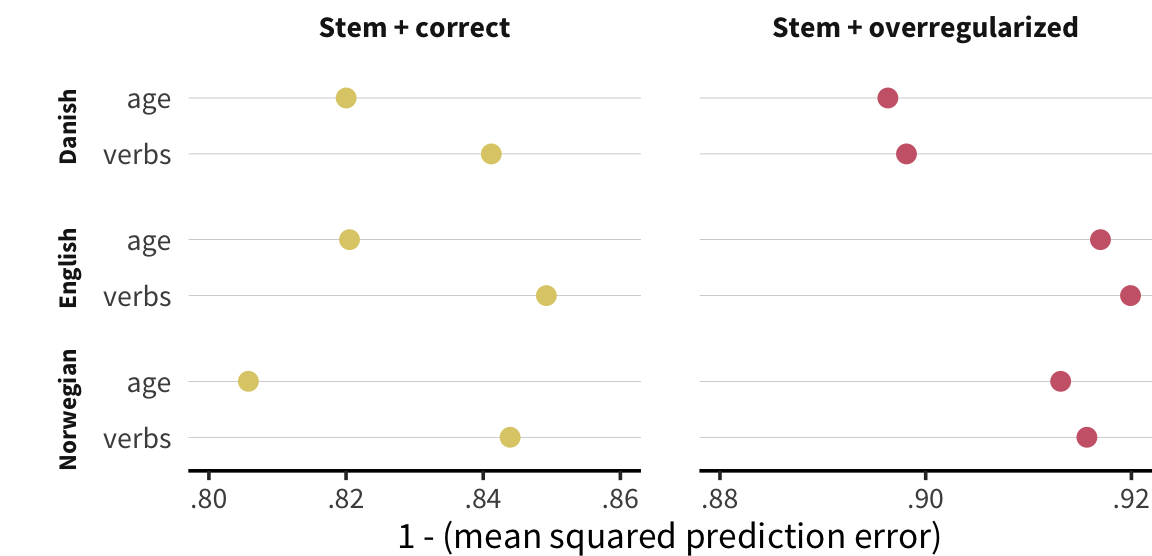
\includegraphics[width=0.8\textwidth]{03-cdi-overreg/plots/models-mse} 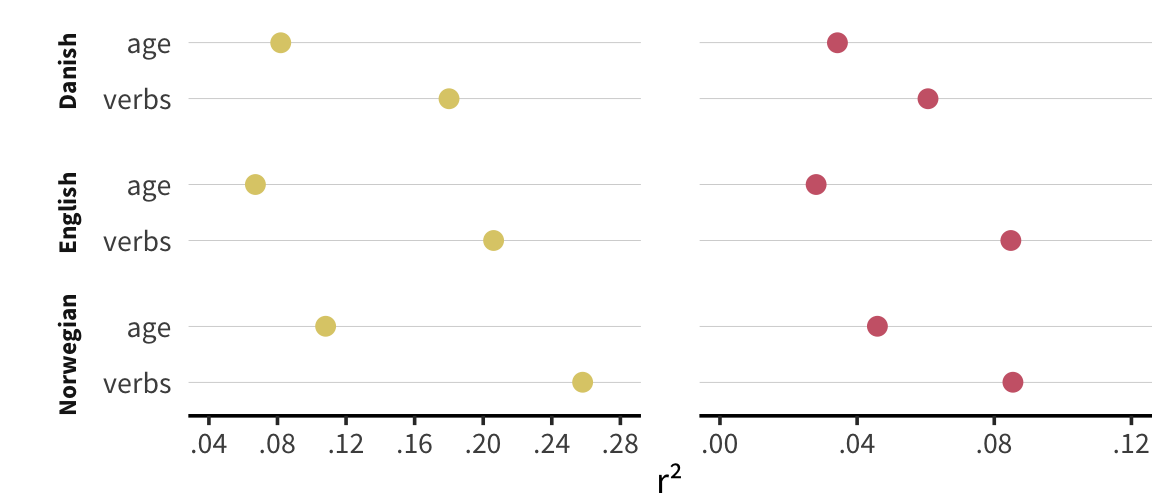
\includegraphics[width=0.8\textwidth]{03-cdi-overreg/plots/models-rsq} 

}

\caption{Model comparison metrics (top: mean squared prediction error, bottom: adjusted r²) for models predicting correct inflection (left) and overregularization (right) from only age or only verb vocabulary size.}\label{fig:overreg-modelcomp}
\end{figure}

The first question we want to address with these datasets is whether morphology is driven more by vocabulary or by age. To examine this, for each language and measure (\texttt{stem\ +\ correct} and \texttt{stem\ +\ overregularized}), we fit two different mixed-effect logistic regressions (with a random effect of item), predicting whether each child inflects or overregularizes just from age or just from verb vocabulary size. We then compare the two models on how much variance they explain and on how robust their predictions are by performing 10-fold cross-validation over the dataset and computing mean sample prediction error.

Figure~\ref{fig:overreg-modelcomp} shows the MSE (mean sample prediction error) and \(r^2\) values for each model. The verbs-only models perform better at out of sample prediction than the age-only models in both \texttt{stem\ +\ correct} (MSE averaged over languages is 0.16 for verbs and 0.18 for age) and in \texttt{stem\ +\ overregularized} (0.089 for verbs and 0.091 for age). They also explain more variance in both correct inflection (\(r^2\) averaged over languages is 21\% for verbs and 8.6\% for age) and overregularization (7.7\% verbs, 3.6\% age).

\hypertarget{analysis-2-vocabulary-and-age}{%
\subsection{Analysis 2: Vocabulary and age}\label{analysis-2-vocabulary-and-age}}

Moving beyond a binary decision between vocabulary and age, we want to see how both of them affect morphology when considered together. We again fit mixed-effects logistic regressions predicting correct inflection and overregularization, but now with terms for age, linear effect of verb vocabulary, quadratic effect of verb vocabulary, and interactions between age and linear/quadratic verb vocabulary terms. The complex models with this full set of predictors are justified by the same cross-validation method described in Analysis 1 when compared to ones for each subset of predictors. The full model is specified as:

\begin{footnotesize}
\texttt{says $\sim$ verbs + verbs² + age + age \& verbs + age \& verbs² + (1 + verbs + age | item)}
\end{footnotesize}

\begin{figure}

{\centering 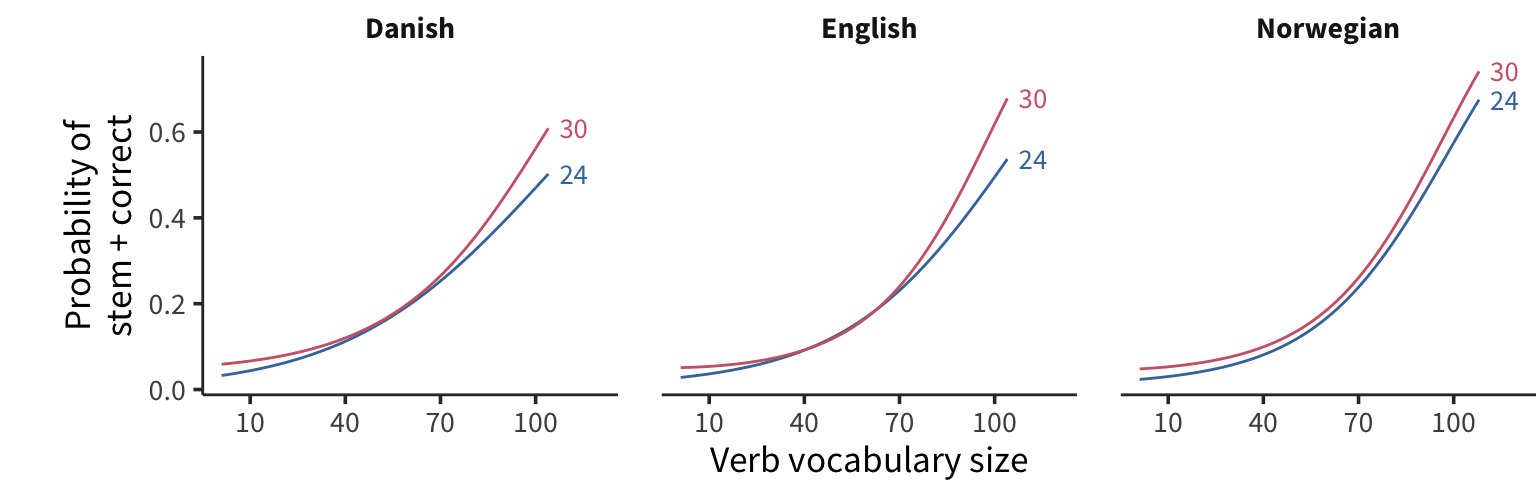
\includegraphics[width=\textwidth]{03-cdi-overreg/plots/correct-traj} 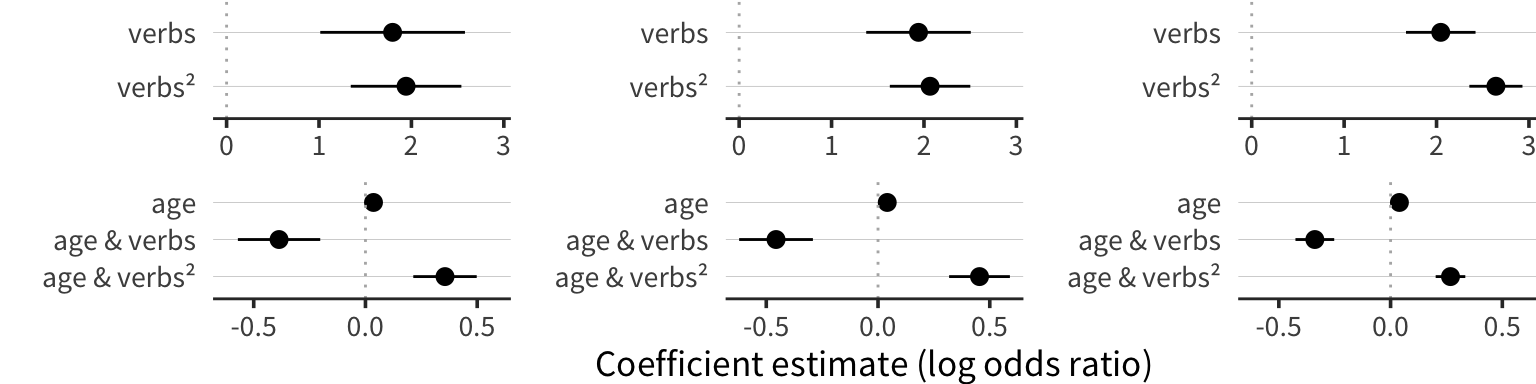
\includegraphics[width=\textwidth]{03-cdi-overreg/plots/correct-coef} 

}

\caption{Model fit probabilities (top) and coefficients (bottom) for full model predicting correct inflection from age and vocabulary.}\label{fig:overreg-correct}
\end{figure}

\textbf{Correct inflection}. Figure~\ref{fig:overreg-correct} shows the coefficients from the \texttt{stem\ +\ correct} models, as well as model fit probabilities of production at 24 and 30 months. In all three languages, there is a positive linear effect of verb vocabulary, such that children with larger vocabularies are more likely to inflect correctly. For example, a 24-month-old English learning child who knows 20 verbs has a 4.9\% chance of correctly inflecting any one item, while a child who knows 80 verbs has a 31\% chance. There is also a positive quadratic effect of verb vocabulary, meaning that the more verbs a child knows, the stronger the effect of an increase in number of verbs is on the probability of producing \texttt{stem\ +\ correct}. As such, at 20 verbs learning another 10 verbs raises the chance of correctly inflecting by only 1.8 percentage points, while at 80 verbs, learning another 10 verbs raises the chance by 8.9 percentage points.

The effect of vocabulary is also modulated by age. The positive effects of age indicate that older children are more likely to produce stem + correct, even controlling for vocabulary size. A 24-month-old who knows 80 verbs has a 31\% chance of correctly inflecting any given item, while a 30-month-old has a 34\% chance. The negative interactions between age and verb vocabulary indicate that the effect of verb vocabulary is larger for younger children, although the age difference is most prominent at the ends of the vocabulary range.

\begin{figure}

{\centering 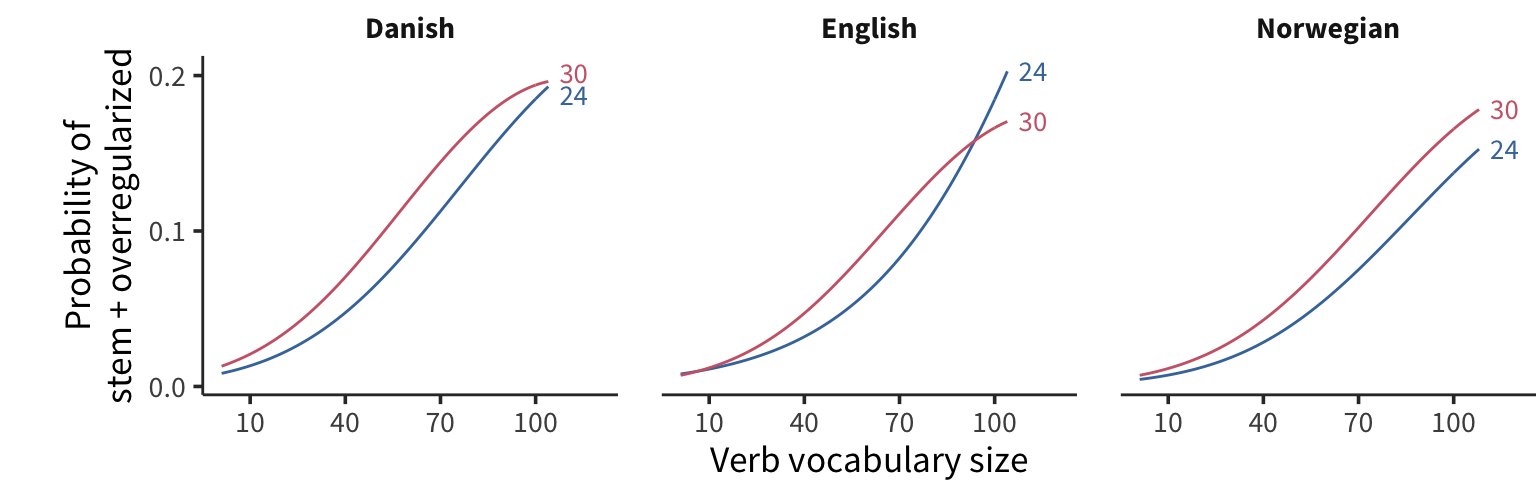
\includegraphics[width=\textwidth]{03-cdi-overreg/plots/overreg-traj} 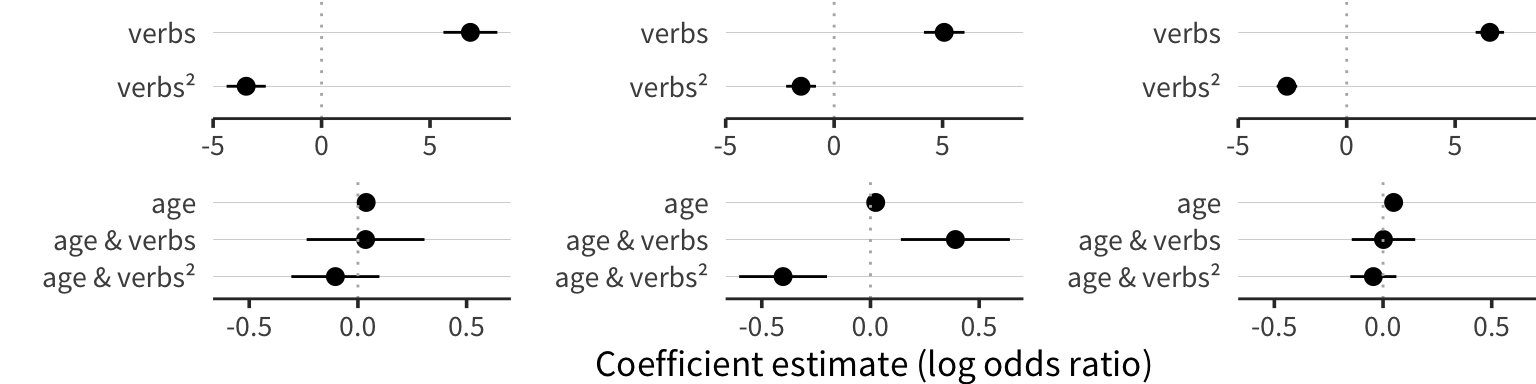
\includegraphics[width=\textwidth]{03-cdi-overreg/plots/overreg-coef} 

}

\caption{Model fit probabilities (top) and coefficients (bottom) for full model predicting overregularization from age and vocabulary.}\label{fig:overreg-overreg}
\end{figure}

\textbf{Overregularization}. Figure~\ref{fig:overreg-overreg} shows the parallel coefficients and predictions for the \texttt{stem\ +\ overregularized} models. As in correct inflection, for overregularization we also see positive linear effects of verb vocabulary (more verbs means more likely to produce stem + overregularized), but we see negative quadratic effects of verb vocabulary (the effect of verb vocabulary decreases with verb vocabulary). A 24-month-old English learning child who knows 20 verbs has a 1.6\% chance of correctly inflecting any one item, while a child who knows 80 verbs has a 11\% chance; at 20 verbs, learning another 10 verbs raises the chance of overregularizing by only 0.67 percentage points, while at 80 verbs, learning another 10 verbs raises the chance by 3.4 percentage points.

We again see positive effects of age: in this age range, older children are more likely to overregularize than younger children, controlling for vocabulary size. A 24-month-old who knows 80 verbs has a 11\% chance of overregularizing any given item, while a 30-month-old has a 13\% chance. The interactions between age and verb vocabulary are small and not significant in Danish and Norwegian, and they appear to be artifactual in English due to data sparsity at the high end of the vocabulary range.

\hypertarget{discussion-1}{%
\subsection{Discussion}\label{discussion-1}}

First, we find that morphology learning is strongly related to vocabulary size, more than to age. This supports morphology learning being coupled to lexical learning (or both being coupled to general language ability), rather than developing as separate competences.

Second, the relation between morphology and vocabulary is modulated by age. For two children with the same vocabulary size, the older is more likely both to correctly inflect and overregularize. Additionally, the effect of vocabulary on both measures decreases with age. This suggests that there are developmental changes that affect morphological ability over and above vocabulary.

Our models also provide an estimate of the propensity of each individual verb to be correctly inflected and to be overregularized. In future work, we plan to explore how properties of individual verbs influence these tendencies and what consequences that has to theories of morphology learning.

By mapping developmental change across large samples and multiple languages, we paint an empirical picture that constrains theories of the mechanisms underlying morphology learning.

\hypertarget{time-course-of-overregularization}{%
\section{Time course of overregularization}\label{time-course-of-overregularization}}

Next, we ask whether individual children's overregularization trajectories can paint a clearer picture of the overall developmental time course of overregularization. We again use a large sample of CDI data of overregularization items, but now for longitudinal CDI administrations. We analyze plural noun morphology and past tense verb morphology in two languages, American English and Norwegian. These data allow us to examine changes in generalization across individuals. Since observations are sparser in the English data than the Norwegian, we pursue slightly different approaches in our analysis.

\hypertarget{analysis-1-english}{%
\subsection{Analysis 1: English}\label{analysis-1-english}}

In the American English dataset, out of children who overregularize at least one item, there are 85 with three longitudinal administrations, 2 with four administrations, and none with more than that. For each child, we compute the proportion of items that they are reported to overregularize at each timepoint. We then compare their three overregularization values -- youngest, middle, and oldest (with the two middle values averages for the four administration children). We categorize their overregularization trajectory as:

\begin{itemize}
\tightlist
\item
  \textbf{increase} (\texttt{/}) if youngest to middle \emph{stays the same} or \emph{increases} and middle to oldest \emph{stays the same} or \emph{increases}
\item
  \textbf{decrease} (\texttt{\textbackslash{}}) if youngest to middle \emph{stays the same} or \emph{decreases} and middle to oldest \emph{stays the same} or \emph{decreases}
\item
  \textbf{recovery} (\texttt{Λ}) if youngest to middle \emph{increases} and middle to oldest \emph{decreases}
\item
  \textbf{retreat} (\texttt{V}) if youngest to middle \emph{decreases} and middle to oldest \emph{increases}
\end{itemize}

Figure \ref{fig:overreg-eng-longs-plot} shows the trajectories of each child, grouped by this classification. For both nouns and verbs, the vast majority of children (72\% and 84\%, respectively) \textbf{increase} in overregularization over this age range, a substantial minority (17\% and 16\%) \textbf{recover} from overregularization, and very few \textbf{decrease} or \textbf{retreat}. So we see that by 30 months, most children who have shown any sign of overregularization to date are continuing to overregularize more and more, while some are recovering from an earlier peak rate.

\begin{figure}

{\centering \includegraphics[width=\textwidth]{thesis-mikabr_files/figure-latex/overreg-eng-longs-plot-1} 

}

\caption{Empirical overregularization trajectories for American English children with at least three observations, categorized by overall shape.}\label{fig:overreg-eng-longs-plot}
\end{figure}

\hypertarget{analysis-2-norwegian}{%
\subsection{Analysis 2: Norwegian}\label{analysis-2-norwegian}}

Because longitudinal data are so much more plentiful in the Norwegian dataset, we can quantify children's trajectories more rigorously. We analyze the 449 children who overregularize at least one item and have at least 4 administrations. For each child, we fit a two logistic regressions predicting how many items they overregularize from their age, one with a linear effect of age and one with both linear and quadratic effects of age. We also fit the parallel set of model using productive vocabulary size, rather than age, as the predictor. We then select the model that fits the data better (i.e.~has the lower AIC) and classify each child's trajectory as:

\begin{itemize}
\tightlist
\item
  \textbf{increase} (\texttt{/}) if the best fit model is \emph{linear} and the effect of age/vocabulary is \emph{positive}
\item
  \textbf{decrease} (\texttt{\textbackslash{}}) if the best fit model is \emph{linear} and the effect of age/vocabulary is \emph{negative}
\item
  \textbf{recovery} (\texttt{Λ}) if the best fit model is \emph{quadratic} and the quadratic effect of age/vocabulary is \emph{negative}
\item
  \textbf{retreat} (\texttt{V}) if the best fit model is \emph{quadratic} and the quadratic effect of age/vocabulary is \emph{positive}
\end{itemize}

There are not sufficient datapoints per child to compare the effects of vocabulary and age, so we examine both separately. These classifications are analogous to the three datapoint ones from the English data, but are taking advantage of the higher density in Norwegian to have smoothed trajectories and model-based estimates.

Figure \ref{fig:overreg-nor-groups-age} shows each child's trajectory over age, grouped by these classifications. Figure \ref{fig:overreg-nor-groups-vocab} shows the parallel trajectories over vocabulary size. In this dataset, which extends to 36 months, many more children exhibit \textbf{recovery} trajectories for both nouns and verbs: over age, 47\% and 49\%; over vocabulary, 42\% and 39\%. Correspondingly, fewer children exhibit \textbf{increase} trajectories: over age, 44\% and 46\%; over vocabulary, 50\% and 57\%. As such, there is an approximately even split between the two types of trajectories, both over age and over vocabulary. While the English and Norwegian data may differ in a variety of ways, it's plausible that the difference reflects that many children are recovering from overregularizing between 30 and 36 months (an age range that is not represented in the English dataset).

\begin{figure}

{\centering \includegraphics[width=\textwidth]{thesis-mikabr_files/figure-latex/overreg-nor-groups-age-1} 

}

\caption{Model fit overregularization trajectories over age for Norwegian children with at least 4 observations, categorized by overall shape.}\label{fig:overreg-nor-groups-age}
\end{figure}

\begin{figure}

{\centering \includegraphics[width=\textwidth]{thesis-mikabr_files/figure-latex/overreg-nor-groups-vocab-1} 

}

\caption{Model fit overregularization trajectories over productive vocabulary size for Norwegian children with at least 4 observations, categorized by overall shape.}\label{fig:overreg-nor-groups-vocab}
\end{figure}

Additionally, we see evidence that trajectory shape is correlated between nouns and verbs: out of the children who have \textbf{recovery} \emph{noun} trajectories, 62\% also have \textbf{recovery} \emph{verb} trajectories; conversely, out of the children who have \textbf{increase} \emph{noun} trajectories, 59\% also have \textbf{increase} \emph{verb} trajectories (see Figure \ref{fig:overreg-nor-lexcat-plot}).

\begin{figure}

{\centering \includegraphics[width=0.65\linewidth]{thesis-mikabr_files/figure-latex/overreg-nor-lexcat-plot-1} 

}

\caption{Proportion of children exhbiting each verb overrregularization trajectory type as a function of noun overregularization trajectory type.}\label{fig:overreg-nor-lexcat-plot}
\end{figure}

\begin{figure}

{\centering \includegraphics[width=\textwidth]{thesis-mikabr_files/figure-latex/nor-recovery-1} 

}

\caption{Distribution of children's ages (left) and vocabulary sizes (right) at peak overregularization. Each point represents an individual child, with its size reflecting the number of observations per child. Boxes show the means and bootstrapped 95\% confidence intervals of the distributions.}\label{fig:nor-recovery}
\end{figure}

\begin{figure}

{\centering \includegraphics[width=\textwidth]{thesis-mikabr_files/figure-latex/nor-recovery-lexcat-1} 

}

\caption{Correlation between children's ages (left) and vocabulary sizes (right) at peak overregularization of nouns vs. verbs. Each point represents an individual child, with its size reflecting the number of observations per child. Lines show linear regression fit.}\label{fig:nor-recovery-lexcat}
\end{figure}

Lastly, for a more detailed look at recovery from the overregularization, we examine the trajectories of the 289 Norwegian children that have recovery-type trajectories for nouns and/or verbs. For each child's trajectory, we find the age and the vocabulary size at their overregularization peak -- the point where the child was overregularizing the largest number of items. The distributions of these ages and vocabularies are shown in Figure \ref{fig:nor-recovery}. The mean age that marks the start of recovery is 27.9 for nouns and 29.2 for verbs. The mean vocabulary size that marks the start of recovery is 0.63 (461 items) for nouns and 0.71 (519 items) for verbs. Additionally, both ages and vocabulary sizes at peak overregularization are correlated between nouns and verbs (Figure \ref{fig:nor-recovery-lexcat}): \(\rho\)=0.68 for age and \(\rho\)=0.69 for vocabulary size.

\hypertarget{discussion-2}{%
\subsection{Discussion}\label{discussion-2}}

Examining longitudinal data on overregularization errors in English and Norwegian, we found that the majority of children who overregularize at all tend to continue to overregularize an increasing number of items between 16 and 30 months. A substantial minority of children show recovery from overregularization, particularly between 30 and 36 months. For these children, the onset of recovery from overregularization occurs on average at around 28 months or 440 words, with verb recovery occurring later than noun recovery. Whether children's overregularization increases or recovers over the range is correlated between nouns and verbs, and for children who recover from overregularization, the age and vocabulary at which they begin to recover is correlated between nouns and verbs.

\hypertarget{cdi-overreg-conclusion}{%
\section{Conclusion}\label{cdi-overreg-conclusion}}

This chapter examined overregularization data in English, Danish, and Norwegian. A central takeaway from our analyses is that there is tremendous heterogeneity in these data -- some children are never reported to overgeneralize within the age range of the sample, while others do substantially more. Of the children who do overregularize, there is large variety in both the shape and timing of their overregularization trajectories. As such, there is not a set course of morphological development across children, both in terms of their age and vocabulary.

Within this heterogeneity, however, we discovered several interesting patterns.
First, we found that overregularization is driven more by vocabulary than by age, but that there is an effect of age over and above vocabulary. This suggests children make morphological abstractions on the basis of their lexicon, as opposed to at a set developmental timepoint, but that there are age-related processes beyond lexical development also at play. These could be either maturational or experiential, and either domain-general (like working memory) or language-specific (like grammatical knowledge).

Second, individual children's trajectories can be fruitfully categorized by overall shape, leading to the observation that for children who overregularize, approximately half begin recovery towards correct inflection at around 30 months and half continue to overregularize more and more through 36 months. Individual children's overregularization also tends to pattern similarly for nouns and verbs.

One important caveat to these findings is the possibility that parents are less keen observers of morphological generalization than they are of vocabulary growth more broadly. It is possible that the lack of systematicity we observed is due to inconsistency in which parents report overgeneralization -- perhaps only some parents are sensitized to the somewhat meta-linguistic observation that their child is using a frequent ending incorrectly (e.g., \emph{foots}). This kind of bias would be consistent with the noun-verb overregularization correlation we observed. Only systematic validation outside of the CDI would truly dispel this worry.

\hypertarget{prod-comp}{%
\chapter{Similarities and differences among models of productivity}\label{prod-comp}}

\hypertarget{introduction-2}{%
\section{Introduction}\label{introduction-2}}

One of the central challenges facing a child learning language is when and how
to form generalizations beyond their exact input. An English-learning child
needs to infer, for example, that not only do many verbs that they have heard
form the past tense by adding +/\textipa{d}/ to the stem (\emph{talk} \(\rightarrow\)
\emph{talked}, \emph{bark} \(\rightarrow\) \emph{barked}) but that novel forms can do so as well
(\emph{glip} \(\rightarrow\) \emph{glipped}). At the same time, the child needs to encode
that there are exceptions to this pattern and learn their form (\emph{go}
\(\rightarrow\) \emph{went}). The question of how learners come to know which units in
their language generalize under what conditions in the face of ambiguous,
exception-riddled evidence can be called the \emph{problem of productivity}
\citep{odonnell2015}.

While the problem of productivity has been at the heart of the study of language
for centuries \citep{bauer2001}, there is an increasing consensus that the
distribution of linguistic units -- that is, its pattern of usage of words,
stems, affixes, etc. across different contexts -- plays a central role
\citep{baayen2009, bauer2005, odonnell2015, yang2016}. In particular, three recent
theories -- Baayen's hapax-based approach \citep{baayen1993, baayen2001, baayen2009}, Yang's tolerance principle \citep{yang2005, yang2010, yang2016}, and
O'Donnell's productivity and reuse tradeoff \citep{odonnell2011, odonnell2015, odonnell2009} -- are distinguished by their theoretical foundations,
mathematical precision, empirical coverage, and contact with linguistic theory.

The theories make fundamentally different psychological assumptions in terms of
whether cognitive computations are performed sequentially or in parallel and
whether linguistic representations are probabilistic or deterministic. These
differences represent opposing views about the nature of linguistic computation.
Thus, a crucial scientific goal is to isolate and study linguistic phenomena in
which these different approaches lead to differing empirical predictions. Our
work aims to examine these three leading theories of morphological productivity
and delineate both the substantive similarities and the crucial differences
among their assumptions and predictions.

To perform this evaluation, we study variants of these models for which
inferences are directly comparable in an artificial domain that captures the
essential features of the problem of productivity. We perform a series of
analyses that show that the models make systematically differing predictions.
Specifically, we examine three dimensions for which we predict there to be
informative differences between these models: number of types, token counts and
irregular ranks, and rule cost.

In the rest of this paper, we first lay out the problem of productivity as
formalized in this work. We then delineate the representational and
distributional assumptions and properties of each model. Next, we describe the
the three dimensions listed above in terms of the background for their
importance and the predictions we have about their effects on the models. We
then specify the designs of our simulations and show their results. Finally, we
conclude by connecting our model comparisons to future empirical investigations
that will enable adjudication between the theories.

\hypertarget{setup}{%
\section{Setup}\label{setup}}

\hypertarget{learning-problem}{%
\subsection{Learning problem}\label{learning-problem}}

Consider a given morphological system, for example, the much-studied English
past tense. Verbs are inflected to form the past tense using a variety of
morphological processes. For the purposes of this work, we refer to any such
process as a \emph{transformation}, a function that takes a stem and returns its
inflected form. With respect to a certain transformation (e.g.~\textsc{stem}
\(\rightarrow\) \textsc{stem} + /\textbackslash textipa\{d\}/), some verbs are \emph{regular} (their
inflected form matches the application of the transformation, e.g.~\emph{use}
\(\rightarrow\) \emph{used}) and some are \emph{irregular} (their inflected form does not
match the application of the transformation, e.g.~\emph{go} \(\rightarrow\) \emph{went,} not
\emph{go} \(\rightarrow\) \emph{goed}).

To isolate the problem of productivity, we presuppose that the learner has
matched up bases with their inflected forms and isolated the potentially
productive transformation, i.e.~we set aside the problem of rule discovery and
focus on productivity inference. The task for any learner or model is then to
determine for each transformation, whether to use it productively, i.e.~whether
to apply it to novel stems. For example, consider a toy corpus of the English
past tense:

\vspace{1em}
\begin{tabular}{llll}
\hline
\textbf{verb} & \textbf{stem} & \textbf{transformation} & \textbf{count} \\
\hline
% go & \textsc{stem} $\rightarrow$ went & $c_\text{go}$ \\
% walk & \textsc{stem} $\rightarrow$ \textsc{stem} + /d/ & $c_\text{walk}$ \\
% run & \textsc{stem} $\rightarrow$ ran & $c_\text{run}$ \\
% use & \textsc{stem} $\rightarrow$ \textsc{stem} + /d/ & $c_\text{use}$ \\
% bark & \textsc{stem} $\rightarrow$ \textsc{stem} + /d/ & $c_\text{bark}$ \\
go & /\textipa{gow}/ & \textsc{stem} $\rightarrow$ \textipa{wEnt} & $c_\text{go}$ \\
walk & /\textipa{wOk}/ & \textsc{stem} $\rightarrow$ \textsc{stem} + /\textipa{d}/ & $c_\text{walk}$ \\
run & /\textipa{\*r2n}/ & \textsc{stem} $\rightarrow$ \textipa{\*raen} & $c_\text{run}$ \\
use & /\textipa{juz}/ & \textsc{stem} $\rightarrow$ \textsc{stem} + /\textipa{d}/ & $c_\text{use}$ \\
play & /\textipa{plej}/ & \textsc{stem} $\rightarrow$ \textsc{stem} + /\textipa{d}/ & $c_\text{play}$ \\
\hline
\end{tabular}
\vspace{1em}

Faced with this input, the learner would need to determine whether to treat the
transformation \textsc{stem} \(\rightarrow\) \textsc{stem} + /\textbackslash textipa\{d\}/ as
productive and memorize the forms \emph{go/went} and \emph{run/ran}, or to not treat it as
productive and memorize all five forms.

Inferences about productivity could in principle take into account many
distributional properties of the linguistic input. Does it matter how many
regular and irregular verbs there are? Does it matter how many times each verb
occurs in the corpus? Does it matter if irregulars tend to be more frequent than
regulars, or \emph{vice versa}? Theories of productivity have proposed various
distributional information sources as the determinants of productivity,
including type frequencies \citep{bybee1995}, token frequencies, single occurrence
frequencies \citep{baayen1993, baayen2001, baayen2009}, number of exceptions
\citep{yang2005, yang2010, yang2016}, and functions of one or more of the above
\citep{aronoff1976, barnwell2010, taatgen2002, odonnell2015}.

\hypertarget{measuring-productivity}{%
\subsection{Measuring productivity}\label{measuring-productivity}}

We define the productivity of a transformation under some model as the
probability of using that transformation productively, i.e.~applying it to a
novel stem. In this view, a model can be thought of as a function that takes a
corpus as input and returns a probability distribution over transformations
given a novel stem. For each model, we define its productivity measure
\(\mathcal{P}^*\) as the probability it assigns to using a target transformation
\(\tau\) given a novel stem \(s^*\) and a corpus \(D\):
\[\mathcal{P}^* = P(\tau\, |\, s^*,D)\]

We will be defining this quantity for each model under consideration and
computing it under various regimes in our simulations. Any time we refer to the
``productivity'' of a model, we are referring to the corresponding
\(\mathcal{P}^*\).

\hypertarget{models}{%
\section{Models}\label{models}}

In this section, we give an overview of the assumptions of each model and
illustrate its inferences using the toy corpus shown in
Figure~\ref{fig:examples}. We focus on translating the underlying machinery of
each framework to a common language, aiming to make clearer the similarities and
differences among the models and pinpoint the ways in which their predictions
differ. For each model, we define its productivity measure \(\mathcal{P}^*\).

Throughout, we use the notation of the input to a model being a corpus \(D\) of
triplets stem, transformation, count: \((s_i,t_i,c_i)\), where there are \(n\) stems
(in the set of stems \(S = E \cup R\)) of which \(k\) are irregular (in \(E\)) and
\(n-e\) are regular (in \(R\)). Additionally, we designate the counts of the
irregulars as \(c^E_1, c^E_2, \ldots, c^E_e\) and the counts of the regulars as
\(c^R_1, c^R_2, \ldots, c^R_{n-e}\).

\begin{figure*}

% begin not productive
\begin{subfigure}{\textwidth}

  \caption{Target transformation treated as \textbf{not productive}.}
  \label{fig:example_nonprod}
  \vspace{1em}

  \footnotesize

  % begin TP
  \begin{subfigure}[t]{0.4\textwidth}
  \textbf{Sequential searchtime optimization}
    \begin{subequations}
    \begin{empheq}{align*}
    \substack{\text{count(go)}\\ \text{1 step}}\ &\boxed{\irr \text{go, went}}\\[1em]
    \substack{\text{count(walk)}\\ \text{2 steps}}\ &\boxed{\reg \text{walk, walked}}\\[1em]
    \substack{\text{count(run)}\\ \text{3 steps}}\ &\boxed{\irr \text{run, ran}}\\[1em]
    \substack{\text{count(use)}\\ \text{4 steps}}\ &\boxed{\reg \text{use, used}}\\[1em]
    \substack{\text{count(play)}\\ \text{5 steps}}\ &\boxed{\reg \text{play, played}}
    \end{empheq}
    \end{subequations}
  \end{subfigure}
  ~
  % begin PR
  \begin{subfigure}[t]{0.55\textwidth}
  \textbf{Productivity and reuse}
    \begin{subequations}
    \begin{empheq}{align*}
    &\text{inflected forms}\\[0.5em]
    &\boxed{
      \substack{\text{count(go)}\\ \boxed{\irr \text{go, went}}}\
      \substack{\text{count(walk)}\\ \boxed{\reg \text{walk, +/\textipa{d}/}}}\
      \substack{\text{count(run)}\\ \boxed{\irr \text{run, ran}}}\
      \substack{\text{count(use)}\\ \boxed{\reg \text{use, +/\textipa{d}/}}}\
      \substack{\text{count(play)}\\ \boxed{\reg \text{play, +/\textipa{d}/}}}
    }
    \\[1.5em]
    &\text{stems}\\[0.5em]
    &\boxed{
      \substack{1\\ \boxed{\irr \text{go}}}\
      \substack{1\\ \boxed{\reg \text{walk}}}\
      \substack{1\\ \boxed{\irr \text{run}}}\
      \substack{1\\ \boxed{\reg \text{use}}}\
      \substack{1\\ \boxed{\reg \text{play}}}
    }
    \end{empheq}
    \end{subequations}
  \end{subfigure}

\end{subfigure}

% begin productive
\begin{subfigure}{\textwidth}

  \caption{Target transformation treated as \textbf{productive}.}
  \label{fig:example_prod}
  \vspace{1em}

  \footnotesize

  % begin TP
  \begin{subfigure}[t]{0.4\textwidth}
    \textbf{Sequential searchtime optimization}
    \begin{subequations}
    \begin{empheq}{align*}
      \substack{\text{count(go)}\\ \text{1 step}}\ &\boxed{\irr \text{go, went}}\\[1em]
      \substack{\text{count(run)}\\ \text{2 steps}}\ &\boxed{\irr \text{run, ran}}\\[1em]
      \substack{\text{count(+/\textipa{d}/)}\\ \text{rule application}}\ &\boxed{\reg \text{*, +/\textipa{d}/}}
    \end{empheq}
    \end{subequations}
  \end{subfigure}
  ~
  % begin PR
  \begin{subfigure}[t]{0.55\textwidth}
    \textbf{Productivity and reuse}
    \begin{subequations}
    \begin{empheq}{align*}
      &\text{inflected forms}\\[0.5em]
      &\boxed{
        \substack{\text{count(go)}\\ \boxed{\irr \text{go, went}}}\
        \substack{\text{count(run)}\\ \boxed{\irr \text{run, ran}}}\
        \substack{\text{count(+/\textipa{d}/)}\\ \boxed{\reg \text{*, +/\textipa{d}/}}}
      }
      \\[1.5em]
      &\text{stems}\\[0.5em]
      &\boxed{
        \substack{1\\ \boxed{\irr \text{go}}}\
        \substack{1\\ \boxed{\irr \text{run}}}\
        \substack{\text{count(walk)}\\ \boxed{\reg \text{walk}}}\
        \substack{\text{count(use)}\\ \boxed{\reg \text{use}}}\
        \substack{\text{count(walk)}\\ \boxed{\reg \text{play}}}
      }
    \end{empheq}
    \end{subequations}
  \end{subfigure}

\end{subfigure}

\caption{Representations of example corpus under two different hypotheses.}
\label{fig:examples}

\end{figure*}


\hypertarget{hapax-based-statistical-estimators}{%
\subsection{Hapax-based statistical estimators}\label{hapax-based-statistical-estimators}}

By far the most thoroughly studied and widely used measures of productivity are
Baayen's P**, P* and P \citep{baayen2001}. Because productive affixes frequently
give rise to new words, their word frequency distributions typically contain a
large number of low frequency forms. This observation suggests that a reasonable
estimate of the productivity of an affix might be based on the number or
proportion of low-frequency words associated with the affix. Baayen's statistics
are based on this idea. In particular, all three quantities estimate the
probability of unobserved (i.e., novel) words using the proportion of word types
which appear only once in a corpus (hapaxes). This intuition can be rigorously
justified under several different sets of mathematical assumptions
\citep{baayen2001}. Baayen's P* (\emph{expanding productivity}) corresponds to a direct
estimator of our \(\mathcal{P}^*\).

In particular, for a corpus of \(N\) words, let \(|H\)\textbar{} be the number of words in
the corpus with frequency 1 (hapaxes): \(H = \{s \in S\ |\ c_s = 1\}\); and let
\(|H_R|\) be the number of hapaxes in the corpus that use the target
transformation: \(H_R = \{s \in R\ |\ c_s = 1\}\). P* is then the proportion of
all hapaxes in the corpus that use the target transformation:

\[ \mathcal{P}^*_\texttt{HAPAX} = \frac{|H_R|}{|H|}\]

\hypertarget{tolerance-principle}{%
\subsection{Tolerance principle}\label{tolerance-principle}}

In a series of studies, Yang has developed a theory of productivity known as the
tolerance principle \citep{yang2005, yang2010, yang2016}. Below we describe first
the machinery underlying the tolerance principle, the elsewhere condition serial
search model, and then its analytic form. Our model comparison set includes both
versions.

\hypertarget{elsewhere-condition-serial-search}{%
\subsubsection{Elsewhere condition serial search}\label{elsewhere-condition-serial-search}}

The elsewhere condition serial search (\texttt{ECSS}) framework posits that inflecting
a stem is based on serial search through a frequency-ranked list of forms. If
the stem isn't a found in the list, an ``elsewhere condition'' indicates how to
inflect it. For a given transformation, productivity inferences arise from
comparing two candidate lists, one in which all forms are listed (i.e.~stored)
vs.~one in which only the irregulars are listed and the regulars fall under the
elsewhere condition. These two hypotheses are compared based on their expected
processing times. For the example corpus, Figure~\ref{fig:example_nonprod} shows
the full listing (no rule) representation, where all stems are stored in
descending order of frequency, so the most frequent stem (\emph{go}) requires one
time step, the second most frequent stem (\emph{walk}) requires two time steps, and
so on. Figure~\ref{fig:example_prod} shows the rule representation, where the
regulars are pulled out of this list, so they all require a fixed number of
steps (in this case, 3).

More concretely, for our set \(S\) of \(n\) stem types, let
\(T = t_1, t_2, \ldots, t_n\) be the processing time of each stem. The probability
(normalized token frequency) of a stem \(s\) is given by \(P(s)\), its frequency
rank among all stems is given by \(r_s\), and for exceptions, their frequency rank
among exceptions is given by \(r_e\).

The no rule hypothesis corresponds to the search time of each stem being equal
to its rank among all stems. So the expected processing time \(T_\text{NR}\)
averaged over all stems is given by:

\[ \mathbb{E}[T_\text{NR}] = \sum_{s \in S} P(s)t_s = \sum_{s \in S} P(s)r_s \]

For the rule hypothesis, the processing times of exceptions are equal to their
ranks within the list of exceptions \(t_s = r_e\), while each of the regulars
requires the same number of processing time steps, \(k\), plus the fixed cost
\(\omega\) of applying the rule \(t_s = e + \omega\). So the expected processing
time \(T_\text{R}\) is given by:

\[ \mathbb{E}[T_\text{R}] = \sum_{s \in S} P(s)t_s = \sum_{s \in S} P(s) (\delta_e r_e + (1 - \delta_e)(k + \omega)) \]

Where \(\delta_e\) is an indicator variable that is equal to one if \(s\) is an
exception.

Inference of productivity then comes from comparing the two expected running
times \(\mathbb{E}[T_\text{R}]\) and \(\mathbb{E}[T_\text{NR}]\).

There are multiple possibilities for how this hypothesis selection might be used
to determine \(\mathcal{P}^*\). Given a novel stem, the model could categorically
apply the regular transformation if and only if the rule hypothesis is selected:

\[
\begin{aligned}
\mathcal{P}^*_{\texttt{ECSS}}
&=
  \begin{cases}
    1 & \mathbb{E}[T_\text{R}] < \mathbb{E}[T_\text{NR}] \\
    0 & \text{otherwise}
  \end{cases}
\end{aligned}
\]

Or it could always apply the regular transformation under the rule hypothesis
and select a transformation uniformly at random under the no rule hypothesis:

\[
\begin{aligned}
\mathcal{P}^*_{\texttt{ECSS}}
&=
  \begin{cases}
    1 & \mathbb{E}[T_\text{R}] < \mathbb{E}[T_\text{NR}] \\
    \frac{1}{k+1} & \text{otherwise}
  \end{cases}\\[2ex]
\end{aligned}
\]

Here we use the latter \(\mathcal{P}^*\) for \texttt{ECSS}, in line with \citep{schuler2016}.

\hypertarget{tp}{%
\subsubsection{Analytic tolerance principle}\label{tp}}

Yang makes a number of distributional assumptions that allow for the derivation
of a generally-stated evaluation metric that does not depend on token
frequencies. This simplification requires assuming that:

\begin{enumerate}
\def\labelenumi{(\arabic{enumi})}
\item
  Token frequencies follow the Zipfian distribution (for a stem of rank \(r_s\),
  \(P(s)=\frac{1}{r_sH_n}\) where \(H_n = \sum_{i=1}^n \frac{1}{i}\).
\item
  Irregulars are a random subset of all stems (each stem's probability of
  being irregular is \(k/n\)).
\item
  A random sample from a Zipfian distribution is also Zipfian, so the token
  frequencies of the irregulars also follow the Zipfian distribution. (for a
  stem of rank \(r_e\) among exceptions, \(P(s)=\frac{1}{r_eH_e}\).
\item
  There is no cost associated with rule application (\(\omega=0\)).
\end{enumerate}

With these assumptions about the input, the model yields the threshold that if
\(k\) types are irregular out of \(n\) total, the transformation will be considered
productive if and only if \(k \leq \frac{n}{\log{n}}\). As such, the threshold
depends only on the type frequencies of regulars and irregulars and does not
interact in any way with their token frequencies.

Under the analytic tolerance principle threshold \texttt{TP}, if there is a productive
transformation, it will always be used for novel stems. It is less clear how
this model ought to treat novel stems if there is not a productive
transformation. As above for \texttt{ECSS}, we use a fallback to picking a
transformation uniformly at random:

\[
\mathcal{P}^*_{\texttt{TP}} =
  \begin{cases}
    1 & e \leq \frac{k}{\log{k}} \\
    \frac{1}{e+1} & \text{otherwise}
  \end{cases}
\]

\hypertarget{productivity-and-reuse-tradeoff}{%
\subsection{Productivity and reuse tradeoff}\label{productivity-and-reuse-tradeoff}}

Another theory of productivity is O'Donnell's productivity and reuse tradeoff
\citep{odonnell2011, odonnell2015, odonnell2009}. This approach is based on the
idea that the productivity of linguistic units can be determined by optimizing a
probabilistic trade-off between a pressure to store fewer, more reusable
primitive units and a pressure to account for each linguistic expression in as
few computational steps as possible. These pressures are quantified in terms of
probability and competition is resolved in parallel. To capture this tradeoff,
the productivity and reuse framework makes the following two assumptions.

First, it assumes that the probability of an expression is the product of the
probabilities associated with the use of each lexical item in the derivation of
that expression expression. Since probabilities are numbers between \(0\) and \(1\),
a product of probabilities declines rapidly (geometrically quickly) as the
number of probabilities in the product increases. The more complex a derivation
is, therefore, the smaller its probability will be, on average. Of course, the
exact probability will depend on the probabilities of individual lexical items
in a derivation. If all of the lexical items are very probable, then the
expression will also be more probable. Nevertheless, more complex derivations
will tend to have lower probabilities regardless of the specific lexical items
within them. This assumption creates a bias towards derivations which use fewer
lexical items per expression, in the extreme case perhaps treating entire
expressions as single lexical units.

Second, it assumes that the probability of a lexical item in some context in a
derivation is proportional to the number of times that lexical item was used in
the same context in the derivation of other expressions. This implements a
rich-get-richer scheme: The probability that a lexical item be used will
increase as it is used more. For a given corpus, the fewer items in the lexicon,
the more often (on average) each item will have to be used across derivations
and, thus, the more probable each item will be. Relating the probability of
lexical items to their frequency of use straightforwardly implements the bias
towards smaller lexicons with smaller, more reusable lexical items.

These assumptions lead to a tradeoff. One one hand, the learner could avoid
complex derivation by storing a large number of relatively big lexical items.
While this would minimize the complexity of derivations, each lexical item would
be less reusable across expressions, and thus less probable. On the other hand,
the learner could favor a small number of relatively small lexical items. These
lexical items would be highly reusable across contexts and thus highly probable.
However, many of them would be required to analyze each expression. The best
lexicon is the one which optimizes these competing constraints.

As a consequence of this evaluation metric, productivity is determined by a
complex interplay between type and token frequencies. More regular types would
generally lead to the regular transformation being more likely to be productive
(more forms can be decomposed, meaning more savings from having a table for the
regular transformation). However, this is not necessarily the case, and
interacts with the relative frequencies of the regular and irregular forms. High
token frequency regular forms can actually inhibit the drive toward
productivity, since a high probability of use creates a higher computational
cost. The biggest driver of productivity is a high number of low frequency
regular forms, corresponding to the intuition that the best evidence for the
productivity of a transformation is seeing it used productively, i.e.~applied to
novel forms.

In the general case, a full model based on the productivity and reuse tradeoff
would consider every combination of storage and computation for each form. This
results in a huge hypothesis space and complex inference problem that can be
solved by a stochastic search procedure. Here we take a different approach by
applying the simplifying assumptions described above to the underlying
representations used by the framework. For a given corpus, all forms are
initially treated as computed and are iteratively stored until further storage
does not increase the model's posterior score. This corresponds to a search
through the posterior space that allows for possibilities where some (high
frequency) regulars are stored and/or irregulars computed. The model's
parameters are set to correspond to uninformative priors over storage states.

The productivity metric for this model is then the probability of using the
target transformation given a novel stem, conditioned on the storage state found
by the procedure described above.

\hypertarget{predictions}{%
\section{Predictions}\label{predictions}}

We lay out three key dimension for which we predict the models that we are
comparing to have informative convergences and divergences in their behaviors.
In our simulations, we will quantitatively evaluate these predictions.

\hypertarget{number-of-types}{%
\subsection{Number of types}\label{number-of-types}}

\textbf{Background}. How do productivity inferences about a specific transformation
depend on the overall number of types to which that transformation can apply?
Are transformations with smaller or larger domains able to tolerate more
exceptions while being productive? For the tolerance principle, the productivity
threshold, being \(\frac{n}{\log(n)}\), grows sublinearly as function of \(n\), and
so ``\,`{[}S{]}maller' rules\ldots{} can tolerate a relatively higher number of exceptions.
Large rules are more vulnerable'' \citep[p.~66]{yang2016}. According to Yang, this
property is ``the most surprising, and in my view the most important,
quantitative aspect of the Tolerance Principle'' \citep[p.~66]{yang2016}.

For both productivity and reuse and hapax-conditioned productivity, there is no
straightforwardly necessary relationship between productivity and number of
types, because their productivity inferences depend not just on the overall
number of types but on further properties of the type and token distribution of
regulars and irregulars. But there is a likely relationship such that as you
increase the number of types, under reasonable assumptions about word
frequencies, you are more likely to get more regulars that drive towards
productivity (i.e.~more regular hapaxes for HC, more non-stored regulars for
PR).

\textbf{Predictions}. As such, we expect tolerance to number of irregulars as a
function of number of types to \emph{decrease} for \texttt{TP} and to \emph{increase} for \texttt{PR}
and \texttt{HC}, though possibly in different ways depending on properties of the
corpus setup. For \texttt{ECSS}, to the extent that the more general elsewhere
condition serial search model is well approximated by the assumptions of the
analytic tolerance principle, it should exhibit the same behavior.

\hypertarget{token-counts-and-irregular-ranks}{%
\subsection{Token counts and irregular ranks}\label{token-counts-and-irregular-ranks}}

\textbf{Background}. A key feature of the tolerance principle is its simplicity --
only the numbers of regular and irregular types need to be taken into account,
rather than more complex corpus statistics. However, this property comes about
from making a number of assumptions that allow the full \texttt{ECSS} model to be
simplified into the \texttt{TP} analytic form (as described in Section~\ref{tp}). For
the \texttt{ECSS} measure of productivity, token counts and irregular ranks matter --
they translate into probabilities that figure into the calculation of expected
processing time. But for \texttt{TP}, it is assumed that irregulars are a random subset
of all types and that the token count distributions for all types and for
irregulars specifically are both Zipfian. Yang posits that the \texttt{TP} analytic
form has the necessary explanatory power without necessitating the \texttt{ECSS}
calculation and without dependence on token counts. He also argues that a
``{[}e{]}ven if all the exceptions are in the top half of the \(N\) items, the
threshold\ldots{} will hardly move'' \citep[p.~65]{yang2016}.

For both productivity and reuse and hapax-conditioned productivity, token counts
and irregular ranks are crucial. For \texttt{HC} they determine how many regulars are
in the tail of the word frequency distribution such that they have a count of 1;
for \texttt{PR} they similarly influence how many regulars have low counts and are thus
provide pressure against storage of the regular transformation.

The dependence on token counts and irregular ranks is particularly important to
evaluate given that the relation between frequency and irregularity is an
empirical question. Yang notes that while ``it has often been observed that
exceptions tend to clustered the {[}sic{]} high-frequency region of words\ldots{} the
concentration of English irregular verbs at the very top appears to be an
outlier in a wide range of empirical cases'' \citep[p.~65]{yang2016}. In recent work,
\citet{wu2019} confirmed statistically in a sample of 28 languages the long-standing
observation that higher frequency forms tend to be irregular and that irregular
forms tend to be higher frequency.

\textbf{Predictions}. For \texttt{TP}, only type counts matter and token counts should be
irrelevant. For \texttt{ECSS}, in cases where the derivational assumptions of \texttt{TP} are
satisfied (i.e.~irregulars are random), its behavior should be similar to that
of \texttt{TP}, but when they are altered its behavior may diverge. In contrast, for
\texttt{PR} and \texttt{HC}, token counts and irregulars ranks should both play a role, such
that corpus setups where there are more low frequency regulars should be more
conducive to productivity.

\hypertarget{rule-cost}{%
\subsection{Rule cost}\label{rule-cost}}

\textbf{Background}. The focus of the theory of productivity and reuse is on an
optimization tradeoff between storage and computation, in that there is both a
cost associated with storing items (fewer and more reusable stored units is
better) and a cost associated with applying transformations (fewer computation
steps is better). \texttt{ECSS} also implements an optimization (over expected
processing time), but there is no cost associated with applying a
transformation. However, the underlying machinery behind \texttt{ECSS} includes not
just this ``rule selection'' process but also a ``rule application'' process. Rule
application ``is sensitive to the frequency of the morphological constituent''
\citep[p.~55]{yang2016}, much like \texttt{PR} is sensitive to item frequency. The question
becomes, how does the behavior of \texttt{ECSS} change when there is a non-zero cost
associated with the application of a transformation? How does that relate to the
behavior of \texttt{PR}?

Hapax-conditioned productivity is a statistical estimator, rather than a
cognitive model. As such, it doesn't include a notion of storage or computation
and is omitted from this analysis.

\textbf{Predictions}. We predict that the addition of rule cost will change behavior
of \texttt{ECSS}, such that it behaves more similarly to \texttt{PR} when the rule cost is
higher.

\hypertarget{analyses}{%
\section{Analyses}\label{analyses}}

The goal of our analyses is to investigate how inferences about productivity are
determined by various distributional properties of the input, and to
quantitatively evaluate the predictions described above. To perform this
evaluation, we (1) construct a space of parametrically-varying input corpora,
(2) define two simulation regimes using those corpora, and (3) conduct analyses
using these simulations to investigate the role of each of the three factors
described above.

\hypertarget{corpora}{%
\subsection{Corpora}\label{corpora}}

We consider corpora with one potentially productive target transformation that
applies to a subset of stems. The input to a model is a corpus that consists of
a set of triplets \textless{}\texttt{stem}, \texttt{transformation}, \texttt{count}\textgreater, which gives the count of
the number of times the form given by the combination of that stem and
transformation appears in the corpus.

For all corpora we use a Zipfian distribution of token frequencies, such that
for a stem \(s\) with frequency rank \(r_s\):

\[ P(s) = \frac{1}{r_s H_n}, H_n = \sum_{i = 1}^n \frac{1}{i} \]

These artificially generated corpora are determined by:

\begin{itemize}
\item
  Number of types (\(n\)).
\item
  Number of irregular types (each irregular form is assigned to a unique
  transformation, and all other forms are assigned to the target
  transformation, so \(k\) irregulars corresponds to \(k + 1\) transformations).
\item
  Placement of irregulars among all types in frequency rank. Irregular ranks
  are either a random sample of all ranks or are determined such that the gaps
  between them are given by the Zipfian distribution. As an example, a corpus
  with \(n=10\) and \(k=4\) would have ranks (from first to last) given by
  \texttt{IrIrrIrrrIrrrr} (where \texttt{I} indicates an irregular and \texttt{r} indicates a
  regular).
\end{itemize}

\hypertarget{simulations}{%
\subsection{Simulations}\label{simulations}}

Using this space of corpus parametrizations, we run a set of simulations that
examine the models' behavior under various regimes. We use two types of
simulations, one for computing for productivity values and one for finding
productivity thresholds.

\hypertarget{productivity-values}{%
\subsubsection{Productivity values}\label{productivity-values}}

We generate corpora where \(n\) is fixed to 100, and \(k\) ranges from 0 to
0.8\(\cdot n\). For each irregular ranking method, we directly compute
the \(\mathcal{P}^*\) of each model and examine its value as a function of number
of \(k\).

\hypertarget{productivity-thresholds}{%
\subsubsection{Productivity thresholds}\label{productivity-thresholds}}

We define the target transformation to be productive under a given model if its
\(\mathcal{P}^*>0.5\). For a given \(n\), we define a model's productivity threshold
as the greatest number of irregular types such that the target transformation is
productive. We examine how these productivity thresholds change a function of
\(n\) under each irregular ranking method.

The total number of types ranges between 10 and
100. For each value of \(n\), the possible number of irregulars
ranges from 0 to 0.8\(\cdot n\). For a given value of \(n\), we find the
productivity threshold for each model by finding the number of irregulars \(k\)
such that the model gives productive for \(k\) and non-productive for \(k+1\). For
\texttt{TP} and \texttt{ECSS} this consists of checking every number of irregulars from 0 up
until the model gives non-productive; for \texttt{PR} this consists of doing binary
search over the range of possible numbers of irregulars.

\hypertarget{results-1}{%
\section{Results}\label{results-1}}

\hypertarget{analysis-1-number-of-types}{%
\subsection{Analysis 1: Number of types}\label{analysis-1-number-of-types}}

Across all different simulations, there is a striking difference in the shapes
of productivity threshold curves between \texttt{PR} and \texttt{TP}, as shown in
Figure~\ref{fig:thresholds-ranks}. As the overall number of types increases,
\texttt{PR} can tolerate an \emph{increasing} proportion of irregulars, while \texttt{TP} can
tolerate a \emph{decreasing} proportion of irregulars. \texttt{HC} tolerates a roughly
constant proportion of irregulars. An immediate consequence of this observation
is that under \texttt{TP}, it is challenging to account for morphological paradigms
with a generalization that applies to a minority of types (or even to a majority
less than the \texttt{TP} threshold), but is nevertheless productive. This is famously
the case in the German plural, where there is a transformation that applies to a
tiny minority of nouns, but is used productively. One way to attempt to resolve
this issue is to break down types into subsets that only certain transformations
can apply to, leaving a smaller set over which to determine the productivity of
the minority generalization \citep{yang2016}.

\begin{figure}

{\centering 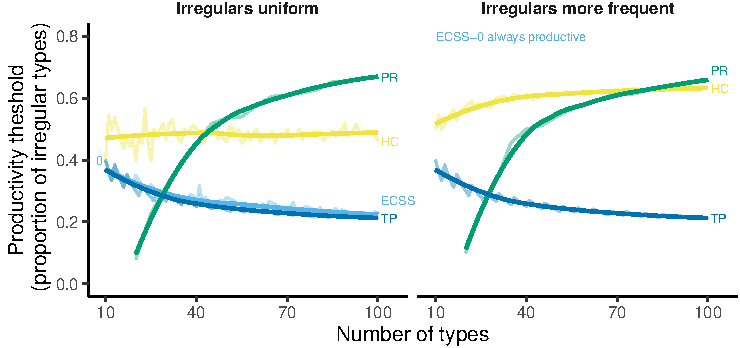
\includegraphics[width=\textwidth]{04-prod-comp/figures/thresholds-ranks-1} 

}

\caption{For each model, curves show the maximum proportion of irregulars for which the regular transformation is inferred to be productive, as a function of total number of types. Panels show different irregular ranking methods.}\label{fig:thresholds-ranks}
\end{figure}

\begin{figure}

{\centering 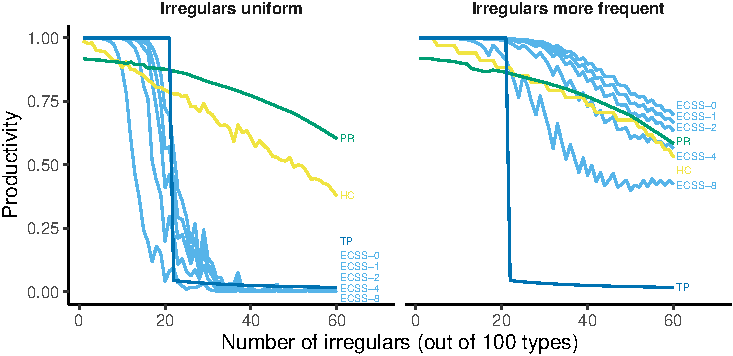
\includegraphics[width=\textwidth]{04-prod-comp/figures/fixed-1} 

}

\caption{For each model, curves show the productivity of the regular transformation as a function of number of irregulars out of a fixed number of types. Panels show different irregular ranking methods.}\label{fig:fixed}
\end{figure}

\hypertarget{analysis-2-token-frequencies-and-irregular-ranks}{%
\subsection{Analysis 2: Token frequencies and irregular ranks}\label{analysis-2-token-frequencies-and-irregular-ranks}}

\textbf{Productivity thresholds}. Figure \ref{fig:thresholds-ranks} also shows the
productivity threshold curves under various exception ranking regimes, with
irregulars ranked uniformly in the left panel and irregulars more frequent in
the right panel.

The tolerance curve for \texttt{PR} is sensitive to the positions of irregulars, in
that \texttt{PR} can tolerate fewer irregulars when they are more frequent than when
they are uniform. However this difference is small, and may be an artifact of
our particular simulation setup.

This analysis reveals a difference in behavior between \texttt{TP} and \texttt{ECSS}. When
irregulars are ranked uniformly, \texttt{ECSS} approximates \texttt{TP} closely. As irregulars
are skewed more towards the high end of the frequency distribution, however,
\texttt{ECSS} systematically deviates from \texttt{TP}, and if irregulars are sufficiently
highly frequent, the productive representation of the data is strictly faster in
processing time that the full listing representation, so the transformation is
\emph{always} treated as productive.

\textbf{Productivity values}. Figure \ref{fig:fixed} shows the productivity
values under various ranking regimes, with irregulars ranked uniformly in the
left panel and irregulars more frequent in the right panel.

Under both irregular ranking methods, the curves for \texttt{PR} and \texttt{HC} are broadly
similar, with a gradual decrease in productivity as the number of irregulars
increases. There is a larger gap between the two when irregulars are uniform as
opposed to when they are more frequent. This is consistent with the idea that
for both \texttt{PR} and \texttt{HC}, productivity is driven primarily by a large number of
low-frequency regulars (directly as hapaxes for \texttt{HC}, indirectly as pressure for
a reusable unit for \texttt{PR}). Their productivity trajectories are thus broadly
similar, but differ less when the irregulars are more frequent, in that the
increasing irregulars don't affect the tail of regulars as much.

Example production trajectories for the words ``dog'' and ``jump'' across languages. Points show the proportion of children producing each word for each one-month age group. Lines show the best-fitting logistic curve. Labels show the forms of the words in each language. For \texttt{TP} and each rule application cost of \texttt{ECSS}, curves
show the maximum proportion of irregulars for which the regular transformation
is inferred to be productive, as a function of total number of types.

\begin{figure}

{\centering 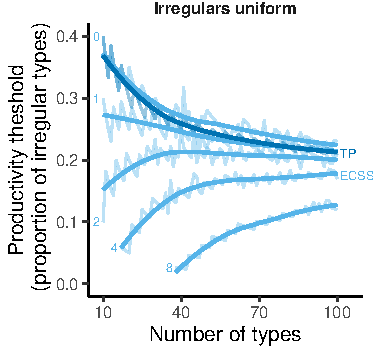
\includegraphics[width=0.5\linewidth]{04-prod-comp/figures/thresholds-ecss-tp-1} 

}

\caption{Example production trajectories for the words ``dog'' and ``jump'' across languages. Points show the proportion of children producing each word for each one-month age group. Lines show the best-fitting logistic curve. Labels show the forms of the words in each language.}\label{fig:thresholds-ecss-tp}
\end{figure}

\hypertarget{analysis-3-rule-cost}{%
\subsection{Analysis 3: Rule cost}\label{analysis-3-rule-cost}}

\textbf{Productivity thresholds}. In Figure \ref{fig:thresholds-ecss-tp}, we show the
productivity threshold curves for \texttt{TP} and for \texttt{ECSS} with rule costs between 0
and 8. As the rule cost increases, the behavior of
\texttt{ECSS} becomes less similar to \texttt{TP} and more similar to \texttt{PR}, with an increasing
proportion of exceptions tolerated as a function of overall number of types.
\texttt{ECSS} without a rule cost, along with \texttt{TP}, encodes a pressure \emph{for}
productivity, in that combining regulars into an elsewhere condition can reduce
their expected search time. The addition of a rule cost adds a pressure
\emph{against} productivity, in that the addition of the elsewhere condition incurs a
separate processing cost. As such the \texttt{ECSS} model can be thought of as encoding
a trade-off between storage and computation similar to that of \texttt{PR}. However,
the threshold curves for \texttt{ECSS} appear to asymptote at a much lower proportion
of irregulars than for \texttt{PR}.

\textbf{Productivity values}. Referring back to the productivity values in Figure
\ref{fig:fixed}, we again see a convergence between the behavior of \texttt{TP} and
\texttt{ECSS} when irregulars are ranked uniformly and for a rule cost of 0, and a
divergence in other settings. Further, we see why in the threshold analysis,
\texttt{ECSS} is always productive when irregulars are frequent, as that is equivalent
to \(\mathcal{P}^*_{\texttt{ECSS-sig}}>0.5\). However, even when the irregulars
are more frequent, the productivity trajectories of \texttt{ECSS} can be differentiated
by rule cost -- the costlier it is to apply the rule, the less productive \texttt{ECSS}
tends to be. \texttt{ECSS} with a non-zero rule cost again more closely resembles \texttt{PR}
than \texttt{TP}, presumably because, as discussed above, it encodes a version of
storage-computation tradeoff.

\hypertarget{prod-comp-conclusion}{%
\section{Conclusion}\label{prod-comp-conclusion}}

We compared and contrasted the assumptions and behaviors of three leading models
of morphological productivity -- the tolerance principle, the theory of
productivity and reuse, and hapax-based estimation. To do this, we generated a
set of parametrically-varying corpora and examined how properties of this
inputs affected the patterns in productivity inferences made by each model.

First, we found a fundamental difference between productivity and reuse on one
hand and the tolerance principle and the more general elsewhere condition
serial search on the other hand. As the overall number of types that a
morphological transformation could apply to increases, \texttt{PR} can tolerate an
\emph{increasing} proportion of irregular types, while \texttt{TP} and \texttt{ECSS} can tolerate
a \emph{decreasing} proportion of irregular types. Commonly studied morphological
systems, for example the English past tense, therefore can't distinguish between
the predictions of these models, because they have a large number of types and
a very low proportion of irregulars.

Second, we isolated several ways in which the analytical form of the tolerance
principle systematically differs from the \texttt{ECSS} model from which it's derived.
The derivation of the tolerance principle crucially involves the assumption
that irregular types a random sample of all types, and for inputs where this
assumption doesn't hold (i.e.~irregulars are skewed towards being higher
frequency), \texttt{ECSS} becomes increasingly prone to productivity.

Additionally, elsewhere condition serial search lends itself to the addition of
a rule cost component, reflecting a tradeoff between storage and computation
rather than an optimization based solely on storage cost. An increasing rule
cost drastically changes the behavior of \texttt{ECSS}, becoming more similar to \texttt{PR}.

An important note about this work is in all of these analyses, the exact values
returned by the models should not be treated as quantitative predictions -- the
input corpora are simulated rather than empirical and the parameter values are
set uninformatively rather than tuned to specific data. Rather, the shapes of
models' predictions within a simulation paradigm gives signatures of their
behavior that can be compared with one another.

Future work could involve finding morphological systems or experimental
paradigms that would enable evaluation of the model differences we isolated
here.

\hypertarget{conclusion}{%
\chapter{Conclusion}\label{conclusion}}

\hypertarget{summary}{%
\section{Summary}\label{summary}}

The studies in this thesis examined children's lexical and morphological development, while aiming to facilitate generalization across children, over development, and among languages.

First, Chapter \ref{aoa-pred} consisted of a study on which properties of words make them easier or harder for children to learn. We found more consistency across languages in these properties than would be expected by chance, reflecting a broad similarity of word learning processes at play cross-linguistically. We also found substantial differences among lexical categories, suggesting different learning routes for content and function words.

Next, Chapter \ref{cdi-overreg} applied similar methodology to investigate patterns in morphological development. Aggregated across children, we found a strong relationship between vocabulary growth and the degree of both correct irregular inflection and overregularization, indicating that lexical and morphological development are tightly coupled. We also saw an effect of age over and above vocabulary, implying that there are age-related processes affecting morphological development that are not captured by vocabulary. For individual children, morphological development patterned in diverse ways but tended to hang together between nouns and verbs.

Finally, Chapter \ref{prod-comp} investigated morphology learning in a language-agnostic way by comparing the predictions of a variety of models of morphological productivity on parametrically-variable corpora. These analyses revealed the different ways in which specific distributional features of the linguistic input -- the type and token counts of regular and irregular forms -- affect the behavior of these models. Understanding these differences is crucial to finding empirical cases that distinguish among theories.

While these studies have led to insights into the processes of language learning, they have not yet involved combining sufficiently rich data with sufficiently well-instantiated models to gain theoretical traction on the nature of morphology learning. As such, I end by laying out a plan for a series of studies that build on work in this thesis by using dense data to evaluate theories of morphology.

\hypertarget{evaluating-theories-of-morphological-development-using-dense-data}{%
\section{Evaluating theories of morphological development using dense data}\label{evaluating-theories-of-morphological-development-using-dense-data}}

Previous work has largely used two data sources on lexical and morphological development: parent-report checklists of children's vocabularies, particularly the CDI \citep{fenson2007}, and transcripts of recordings of children's speech, e.g.~corpora in CHILDES \citep{macwhinney2000}; Speechome \citep{roy2015}; and SEEDLingS \citep{bergelson2016}. While such recordings tend to be collected often per child, they suffer from small sample sizes in terms of the number of children (limited by high transcription cost). Conversely, the standardized and cheap nature of the CDI allows for large sample sizes, but because the CDI is only administered at most every few months, the temporal density of its longitudinal data is limited.

\begin{figure}

{\centering 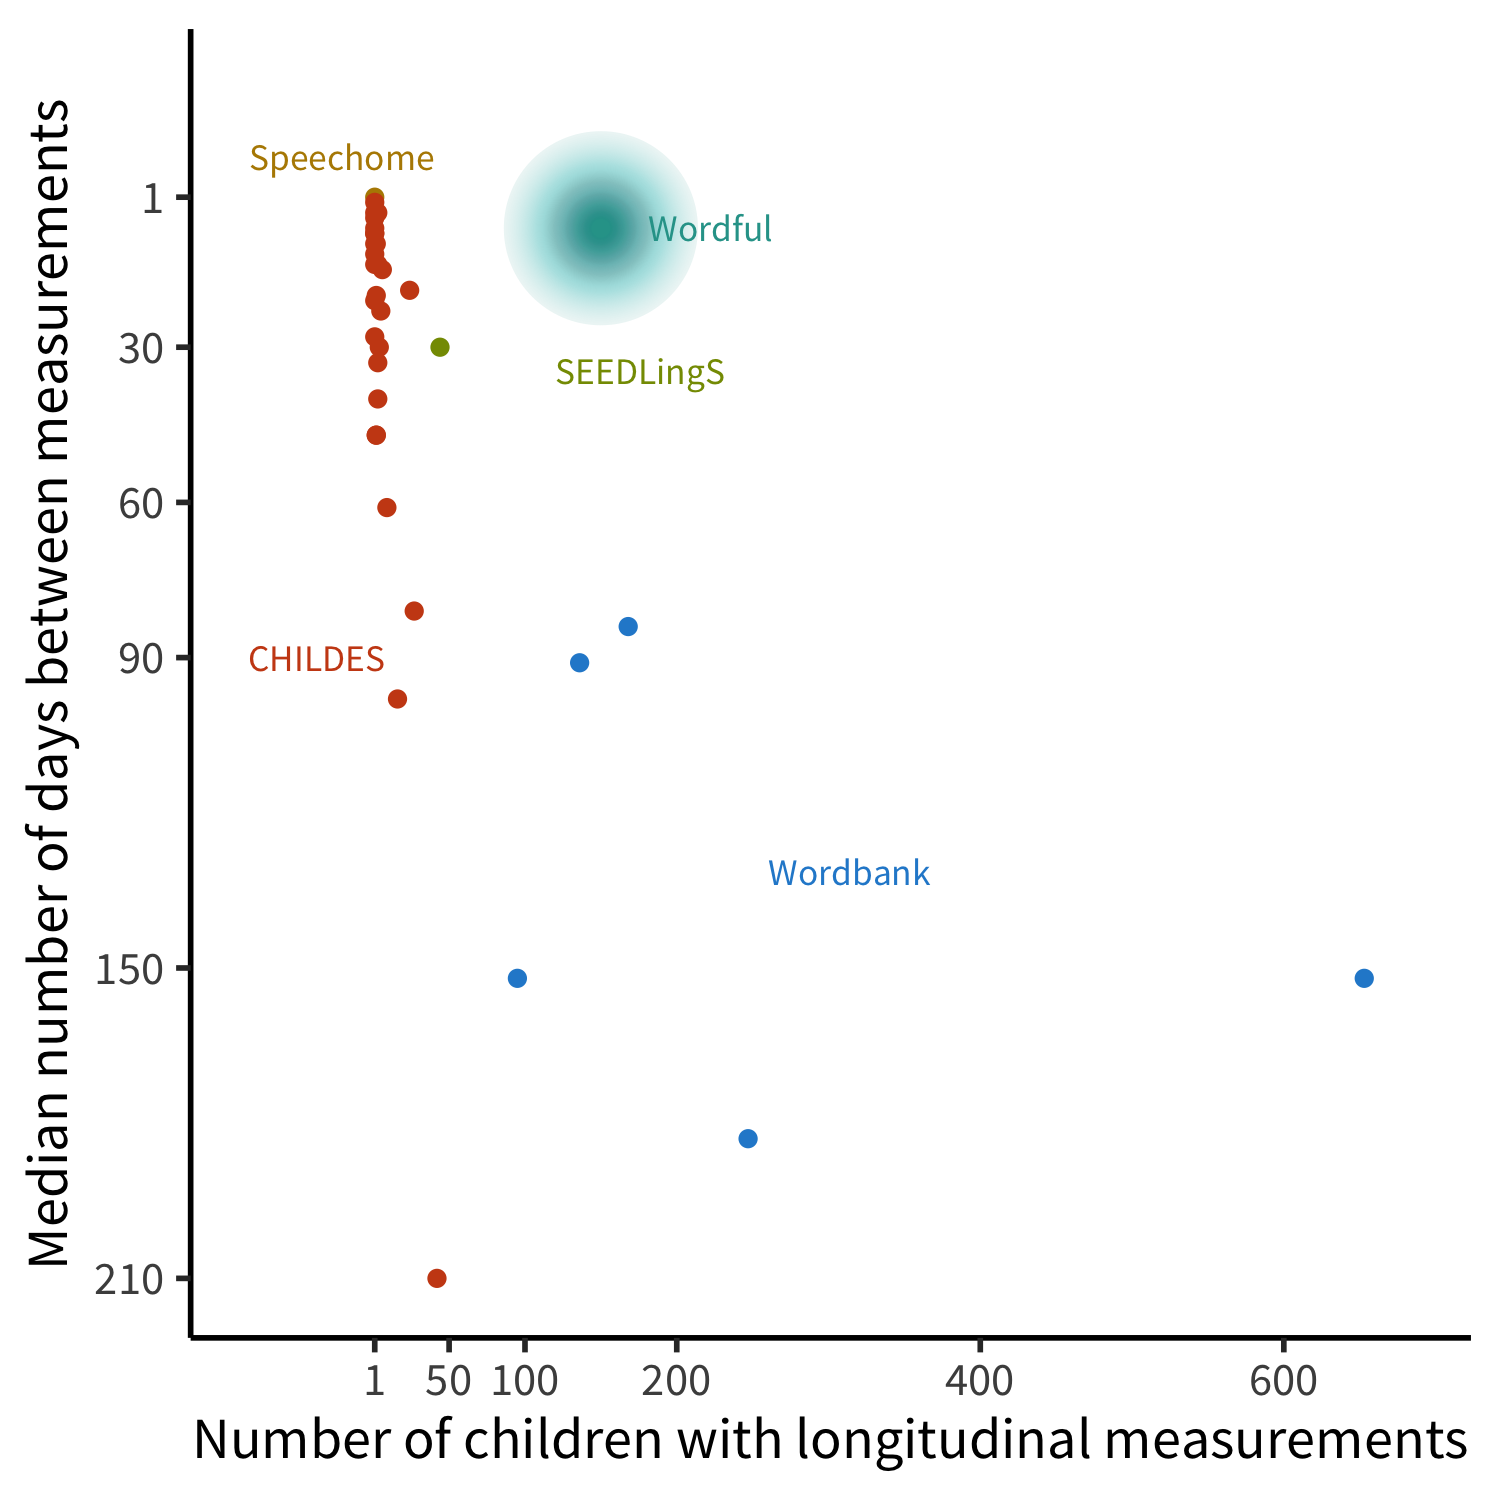
\includegraphics[width=0.6\linewidth]{05-conclusion/corpus_stats} 

}

\caption{Properties of longitudinal corpora of language development data (each point represents one corpus). Wordbank (CDI) data have large N but low temporal density. Naturalistic recordings (e.g., CHILDES, Speechome, SEEDLingS) tend to have high temporal density but low N. Wordful is a novel data collection method that achieves both a large N and high temporal density.}\label{fig:wordful-motivation}
\end{figure}

To address the drawbacks of both CDI data and speech recording samples, we developed a novel data collection method, a smartphone app called Wordful \citep{meylan2019}. Wordful takes advantage of the prevalence of smartphones to collect parental report data scalably and flexibly through a mobile application that parents use to keep track of words in their children's vocabulary as they are produced. This enables the creation of datasets that have both larger sample sizes as in the CDI and higher temporal density as in speech recordings (Figure~\ref{fig:wordful-motivation}). Using Wordful, caregivers report on their child's word production by being presented with cards showing a word and swiping left (no) or right (yes) to indicate whether they've heard their child say that word. Wordful also has a flexible system for sending parents custom questionnaires, such that studies can ask specific questions contingent on a child's vocabulary, age, or other properties.

We plan to use Wordful to create a rich dataset on the morphological development of a large sample of children and use these data to quantitatively evaluate theories of morphology learning. In Study 1, we will conduct a cross-sectional study to assess which properties of words influence their propensity to be overregularized and irregularized. These data will allow us to examine the interplay between memorization and generalization in morphology learning. Then in Study 2, we will conduct a larger, longitudinal study allowing us to characterize the developmental trajectories of (over)generalization for individual children and words. These trajectories constrain the learning mechanisms that children use to make inferences. Finally, Study 3 involves instantiating theories of morphology into comparable computational models, allowing us to test each theory quantitatively on equal footing, and meaningfully compare between proposals using the data Study 2.

\hypertarget{study-1-characterize-generalization-patterns-by-verb}{%
\subsection{Study 1: Characterize generalization patterns by verb}\label{study-1-characterize-generalization-patterns-by-verb}}

\textbf{Motivation: Overregularization}. What does a child saying \emph{goed} or \emph{eated} tell us about what they know? They must have not yet memorized the corresponding correct form (\emph{went} or \emph{ate}) and they must be using some process of generalization to add -\emph{ed} to \emph{go} or \emph{eat}, because \emph{goed} and \emph{ate} are not in the input they have received from adults. So, if children are overall more likely to overregularize \emph{go} (by saying \emph{goed}) than \emph{eat} (by saying \emph{eated}), there must either be something about \emph{went} that makes it less likely to be memorized than \emph{ate}, or something about \emph{go} that makes it more likely to have -\emph{ed} added to it than \emph{eat.} What verb properties affect their propensity to be overregularized, and what do that tell us about these processes of memorization and generalization?

A number of corpus studies have found that less frequent irregulars are more likely to be overregularized \citep{maratsos2000, marcus1992, maslen2004}. Additionally, a corpus analysis of the same data found that irregulars for which the stem has a more dominant vowel than the past tense form are more likely to be overregularized \citep{stemberger1993}. Lastly, an elicited production study with older children found that irregulars that are more phonologically similar to regulars are more likely to be overregularized \citep{marchman1997productivity}.

To the extent that variation in verbs' susceptibility to overregularization can be explained by frequency, the memorization component would likely be responsible, as more frequent forms are more likely to be memorized. Conversely, to the extent that phonological properties of verbs affect their overregularization, generalization must be sensitive to them. So, we can characterize the interplay between memorization and generalization by quantifying the contribution of each of these item-level properties to robust estimates of overregularization rates.

In other words, we plan to rigorously test the previously-observed effect of frequency on overregularization and to extend the effect of phonological similarity from elicited production data to more naturalistic data. In addition, we go beyond previous work by obtaining more robust estimates of overregularization rates for more verbs and assessing the relative contributions of the various factors in a comparable way.

\textbf{Motivation: Irregularization}. What can we learn from a child saying \emph{brang} or \emph{brung} as the past tense of \emph{bring}? Not only have they not memorized \emph{brought}, but they are also extending the irregular patterns of \emph{sing}-\emph{sang} or \emph{cling}-\emph{clung.} Existing corpus data is too sparse to reliably measure rates of irregularization, let alone the differences in these rates for different verbs. While there are not that many verbs that could potentially be irregularized (i.e., that meet the phonological conditions of an irregular pattern) and that young children might know, we can cover them more fully and thus attempt to test the parallel exploratory hypothesis that verbs are more likely to be irregularized if they are less frequent and more phonologically similar to irregulars.

\textbf{Design}. We will recruit parents to use Wordful for approximately one month, targeting those with children that are around 24--36 months (an age range during which children show a range of overregularization behaviors, as observed in Chapter \ref{cdi-overreg}). Once a parent has indicated that their child says a given verb (e.g.~\emph{bring}), we will send them a custom questionnaire in the app, presenting them with a list of possible inflected form(s) of that verb (e.g.~\emph{bringed}, \emph{brang}, \emph{brought}, other, none) and asking them which of those forms their child uses.

We will target these questions for a large set of verbs, both regular and irregular.
Specifically, the target verb list will be chosen to cover a broad range of frequencies and phonological properties, such that we have the power to assess the relative contribution of each factor.
In addition, we will include all verbs that can be irregularized (i.e.~that match the phonological conditions of irregular patterns) and are likely to be known by at least some children in the study age range (as measured by them appearing in children's speech in CHILDES corpora).
For each irregular verb (e.g.~\emph{run}), the options presented in the question will consist of the unchanged stem (\emph{run}), the correct past tense form (\emph{ran}), the overregularization of the stem (\emph{ranned}), the overregularization of the past tense form (\emph{runned}).
In addition, if the verb matches the phonological conditions of an irregular pattern, the application of that pattern will also be included as an option (e.g.~\emph{stang} for \emph{sting}).

\textbf{Analysis}. For each verb (e.g.~\emph{bring}), we will calculate its (1) overregularization rate: how many children over the course of the study were reported to say its overregularized form(s) (\emph{bringed}, \emph{branged}); (2) irregularization rate: how many children over the course of the study were reported to say its irregularized form (\emph{brang}, \emph{brung}).
For each verb, we will estimate its frequency and its phonological similarity to regulars and to irregulars (i.e.~its phonological neighborhood density within each) from child-directed speech in CHILDES corpora.

We will use generalized linear mixed effects models (as the data will have repeat measures of children and of items) to predict verbs' overregularization and irregularization rates from their frequency and phonological similarity to regulars and to irregulars. We will assess the presence of each of these effects, their relative magnitudes, and whether they interact. We expect that both overregularization and irregularization rates will be substantially higher than previously reported, because our data overcome previous sparsity issues. Further, we expect that the relationship between each verb and the structure of the verb lexicon will influence over(ir)regularization rates, in that verbs that are less frequent and/or more phonologically similar to regulars will be overregularized more, and that verbs that are less frequent and/or more phonologically similar to irregulars will be irregularized less. Larger effects of frequency would implicate memorization mechanisms, while larger effects of phonological similarity would implicate generalization mechanisms.

\hypertarget{study-2-relate-learning-trajectories-in-morphology-to-language-development}{%
\subsection{Study 2: Relate learning trajectories in morphology to language development}\label{study-2-relate-learning-trajectories-in-morphology-to-language-development}}

\textbf{Motivation}. What has changed about a child if they had been saying went, but now say goed? What about if they had been saying goed, but now say went? To the extent that these transitions are linked increases in the child's vocabulary, it suggests that generalizations are formed on the basis of the lexicon; to the extent that the changes occur at a given age, it suggests that there is a separate developmental progression at play. In addition, children having periods of overregularizing many words concurrently would be indicative of the operation of a global rule; conversely, different words being overregularized at different times would be indicative of an item-by-item generalization process.

The data from Study 1 does not allow us to make these distinctions, as it is cross-sectional. Thus the goal of Study 2 is to conduct a longitudinal study to measure how each individual child's inflection behavior changes over time and determine what drives these changes. Specifically, we hypothesize that children's tendencies to generalize, overregularize, and irregularize are all more strongly related to their vocabulary size than to their age. While all theories would agree that vocabulary and age are both relevant at least to some extent, evaluating the relative strength of the two factors reveals the extent to which morphology learning is driven by lexical learning or by other developmental changes.

Further, we hypothesize that overregularization and irregularization trajectories vary for individual children and individual items, both in shape and timing, as suggested by previous work \citep{hoeffner1992, plunkett1993}. That is, rather than there being a global period in which all children (or even one individual child) tends to overregularize all items, we predict that only some children and items exhibit U-shaped curves (i.e., first inflect correctly, then overregularize, then inflect correctly again); and that the inflection points for these curves occur at various points in development rather than at the same time. The analyses in this study will evaluate the extent to which trajectories overlap or diverge across children and across items, providing a degree of empirical precision that previous data could not achieve.

\textbf{Design}.
We will recruit parents to use Wordful for approximately six months, targeting children that are 24--30 months at start time (30--36 months at end time), in line with the age range in Study 1.
We will use the same inflection questions as in Study 1, but once the parent has reported on forms of a verb that their child uses, we will ask that question again in two weeks.
We will also use the same items as in Study 1, possibly adjusted based on the results of that study. For example, items that are never (or extremely rarely) produced in the Study 1 data would be excluded from Study 2 to conserve on how much is asked of parents.

\textbf{Analysis}. For each child, we will have a continuous measurement of their age and a rolling estimate of their verb vocabulary size from the word swiping component. We will categorize their responses to inflection questions as indicating that they generalize, overregularize, and/or irregularize each verb, resulting in a rolling estimate of their rates of each behavior. Each child's series of responses for each item will constitute a trajectory for that item.

In the first analysis, we will use generalized linear mixed effects models to predict the estimates of children's rates of generalization, overregularization, and irregularization from their verb vocabulary size and age. In the second analysis, which we will use similar models to categorize each item's trajectory as one of: increase (response(s) of correct form or none followed by response(s) of overregularization); decrease (overregularization, then correct form or none); recovery (correct form, then overregularization, then correct form); retreat (overregularization form, then correct, then overregularization form); or chaotic (no discernible pattern). For each child, we will measure the extent to which they tend to exhibit the same type of trajectories for all items or different types of trajectories for different items. For each child's recovery trajectories, we will estimate the inflection point of the trajectory, indicating the age or vocabulary size at which the child's treatment of the item changes.

For the first analysis, we expect that vocabulary size will be a stronger predictor than age of all inflection behaviors. For the second analysis, we expect that each child's items will vary in the type of overregularization trajectory they display (some U-shaped, others not) and in the timing of the inflection points of those trajectories.

\hypertarget{study-3-using-computational-models-to-distinguish-among-theories-of-morphology}{%
\subsection{Study 3: Using computational models to distinguish among theories of morphology}\label{study-3-using-computational-models-to-distinguish-among-theories-of-morphology}}

\textbf{Motivation}. The analyses from Studies 1 and 2 give broad signatures of the operation of the mechanisms of generalization and memorization by placing morphological development on a continuum between item-based and global inference. To understand these processes more deeply, here we use more detailed learning models to make fine-grained quantitative predictions, and use these to evaluate instantiations of different theories.

A persistent challenge in comparing theories of morphology learning is that models tend not to be tested with clearly differentiated predictions on data that is rich enough to distinguish between them. Because of the difficulty in bridging these gaps, there has been an impasse in argumentation about the predictions of competing theories. For example, dual-route proponents have claimed that connectionist models can only learn rules for which a majority of types are regular \citep[e.g.,][]{marcus1995jcl}, but subsequently many connectionist models have been able to learn systems where even a relatively small proportion of types is regular \citep{hahn2000, nakisa1996, plunkett1997}. Conversely, connectionist modelers have claimed that a dual-route model must exhibit a sharp discontinuity in rate of overregularization \citep[e.g.][]{hoeffner1996}, but whether this is in fact the case is highly dependent on the (unspecified) rule-discovery mechanism of a dual-route account \citep{odonnell2015}. More generally, rigorous testing of different models' predictions, rather than qualitative claims about their behavior, requires grounding them in larger and denser data \citep{meylan2017}.

More recently, a new theory has been proposed for explaining inferences about morphological productivity, namely the tolerance principle \citep{yang2016}. According to this framework, across a wide range of phenomena, children determine whether to form a general rule or store specific forms on the basis of comparison between the sequential search time of these two possible representations. The assumptions made by this model result is a simple heuristic that compares the number of forms that conform to the rule against the number of forms that do not. While this model is claimed to account for children's morphological behavior in both corpus and experimental studies \citep{schuler2016, yang2016}, no study has compared the predictions of the tolerance principle with those of other models on equal footing.

\textbf{Models}. Our goal is to comprehensively evaluate theories of morphology learning. As such, we will include a broad range of the computational modeling frameworks that have been applied to the English past tense. The models we plan to include are the productivity and reuse trade-off \citep{odonnell2011, odonnell2015, odonnell2009, odonnell2011}, the tolerance principle \citep{yang2005, yang2010, yang2016, yang2017}; modern encoder-decoder neural networks \citep{cotterell2016, kirov2018}; and analogical reasoning \citep{daelemans2005, skousen1989}.

\textbf{Training}. The input data for the models will be derived from the Wordful vocabulary data collected in Study 2 (top left box in Figure \ref{fig:wordful-diagram}). For each child, this will consist of a series of timepoints of that child's verb vocabulary, i.e.~the set of verbs that the child has been reported to say. For each of these verbs, we will also obtain an estimate of its token frequency in child-directed speech from CHILDES corpora (a necessary simplification due to the prohibitive cost of measuring individual children's input frequencies). Each model will be fit to each of these by-child timepoints and will then be used to generate predictions about that child's inflections at that time, i.e.~a probability distribution over possible inflected forms of each verb (center box in Figure \ref{fig:wordful-diagram}).

\textbf{Evaluation}. The evaluation data will be based on the inflection data collected in Study 2 (right box in Figure \ref{fig:wordful-diagram}). For each model, the probabilities of the inflected forms that each child was reported to produce at each timepoint will be combined into an overall likelihood of the observed data under that model. To prevent overfitting, regardless of models' parameterization, we will perform cross-validation over verbs and children, training on a subset of the data and evaluating on the held out subset. We will then compare the models' overall prediction error to evaluate which models perform best.

\textbf{Error analysis}. In addition to the overall evaluation, we also want to determine what specific inferential pathways are involved in the models' successes and failures. To do this, we will perform a systematic evaluation of the errors that each model makes, e.g.~whether the model tends to overregularize too much or not enough compared with children and what categories of verbs it tends to inflect differently than children.

\begin{figure}

{\centering 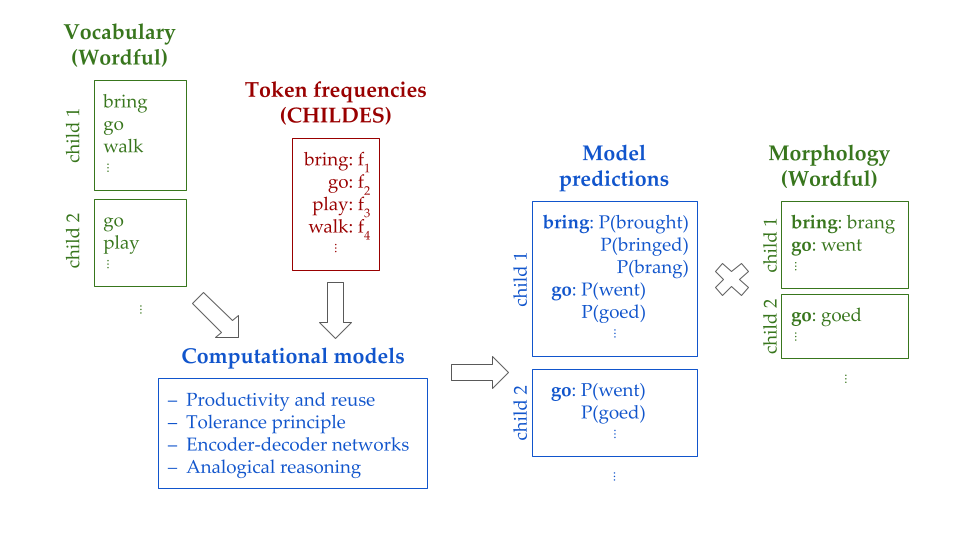
\includegraphics[width=\textwidth]{05-conclusion/sprf_diagram} 

}

\caption{Diagram representing the structure of Study 3. Vocabulary data from Wordful and token frequency information from CHILDES serves as the input to models. The resulting predictions over possible past tense productions are then compared to morphology data from Wordful to evaluate these models.}\label{fig:wordful-diagram}
\end{figure}

\hypertarget{wordful-summary}{%
\subsection{Summary}\label{wordful-summary}}

To learn the structure of words, children need to generalize beyond their input, while simultaneously memorizing exceptions to these generalizations. How do children learn to balance item-specific and global knowledge to generalize without overgeneralizing? We propose a series of studies that entail collecting large, dense data on children's morphological development using a novel app-based data collection method and using these data to quantitatively evaluate theories of morphology learning. In Study 1, we conduct a cross-sectional study to assess which properties of words influence their propensity to be overregularized and irregularized. In Study 2, we conduct a larger, longitudinal study allowing us to characterize the developmental trajectories of (over)generalization for individual children and words. Finally, Study 3 involves instantiating theories of morphology into comparable computational models allowing us to use the data from Studies 1 and 2 to quantitatively test the predictions of theories on equal footing. The combination of dense data and modeling will allow us to advance the empirical and theoretical understanding of morphology learning and of the mechanisms underlying memorization and generalization.

\renewcommand\bibname{References}
  % Thesis added
  \setstretch{1}
  %
  \bibliography{thesis.bib}

\end{document}
